% !TEX program = pdflatex
\documentclass[11pt,a4paper]{article}
\usepackage[utf8]{inputenc}
\usepackage[T1]{fontenc}
\usepackage{lmodern}
\usepackage[a4paper,margin=2.5cm]{geometry}
\usepackage{graphicx}
\usepackage{float}
\usepackage{amsmath}
\usepackage{amssymb}
\usepackage{booktabs}
\usepackage{longtable}
\usepackage{array}
\usepackage{calc}
\usepackage[numbers]{natbib}
\usepackage{hyperref}
\usepackage{url}
\usepackage{xcolor}
\usepackage{caption}
\usepackage{enumitem}
\usepackage{fancyhdr}
\usepackage{lastpage}
\usepackage{titling}
\usepackage{authblk}

\providecommand{\tightlist}{\setlength{\itemsep}{0pt}\setlength{\parskip}{0pt}}

% MDPI metadata commands as no-ops
\newcommand{\firstpage}[1]{}
\newcommand{\pubvolume}[1]{}
\newcommand{\issuenum}[1]{}
\newcommand{\articlenumber}[1]{}
\newcommand{\pubyear}[1]{}
\newcommand{\copyrightyear}[1]{}
\newcommand{\datereceived}[1]{}
\newcommand{\dateaccepted}[1]{}
\newcommand{\datepublished}[1]{}
\newcommand{\history}[1]{}
\newcommand{\publdoi}[1]{}
\newcommand{\doinum}[1]{}
\newcommand{\license}[1]{}
\newcommand{\externaleditor}[1]{}
\newcommand{\academiceditor}[1]{}
\newcommand{\reviewreports}[1]{}
\newcommand{\journalname}[1]{}
\newcommand{\ISSN}[1]{}
\newcommand{\totalpages}[1]{}
\newcommand{\reftitle}[1]{}
\newcommand{\shorttitle}[1]{}
\newcommand{\longtitle}[1]{}

% Title / author / affiliations compatibility
\newcommand{\Title}[1]{\title{#1}}
\newcommand{\Author}[1]{\author{#1}}
\newcommand{\AuthorNames}[1]{}
\date{}
\newcommand{\addressblock}{}
\newcommand{\address}[1]{\gdef\addressblock{#1}}
\newcommand{\corresblock}{}
\newcommand{\corres}[1]{\gdef\corresblock{#1}}

% Abstract and keyword storage
\newcommand{\abstracttext}{}
\makeatletter
\let\oldabstractstart\abstract
\let\oldabstractend\endabstract
\renewcommand{\abstract}[1]{\gdef\abstracttext{#1}}
\makeatother
\newcommand{\keywordtext}{}
\newcommand{\keyword}[1]{\gdef\keywordtext{#1}}

% ORCID links
\newcommand{\orcidA}{\href{https://orcid.org/\orcidauthorA}{\textsc{orcid}}}
\newcommand{\orcidB}{\href{https://orcid.org/\orcidauthorB}{\textsc{orcid}}}
\newcommand{\orcidC}{\href{https://orcid.org/\orcidauthorC}{\textsc{orcid}}}
\newcommand{\orcidD}{\href{https://orcid.org/\orcidauthorD}{\textsc{orcid}}}

% Declarations as titled paragraphs
\newcommand{\dataavailability}[1]{\vspace{1em}\paragraph*{Data Availability.}#1}
\newcommand{\institutionalreview}[1]{\vspace{1em}\paragraph*{Institutional Review Board Statement.}#1}
\newcommand{\informedconsent}[1]{\vspace{1em}\paragraph*{Informed Consent Statement.}#1}
\newcommand{\authorcontributions}[1]{\vspace{1em}\paragraph*{Author Contributions.}#1}
\newcommand{\conflictsofinterest}[1]{\vspace{1em}\paragraph*{Conflicts of Interest.}#1}
\newcommand{\funding}[1]{\vspace{1em}\paragraph*{Funding.}#1}
\newcommand{\acknowledgments}[1]{\vspace{1em}\paragraph*{Acknowledgments.}#1}
\newcommand{\useofartificialintelligence}[1]{\vspace{1em}\paragraph*{Use of Artificial Intelligence Tools.}#1}

% Ensure \maketitle also prints address, abstract, keywords
\makeatletter
\let\oldmaketitle\maketitle
\renewcommand{\maketitle}{%
  \oldmaketitle
  \ifx\addressblock\@empty\else
    \vspace{0.5em}%
    {\small\noindent\addressblock\par}%
  \fi
  \ifx\corresblock\@empty\else
    \vspace{0.3em}%
    {\small\noindent\corresblock\par}%
  \fi
  \ifx\abstracttext\@empty\else
    \vspace{1em}%
    \oldabstractstart\abstracttext\oldabstractend
  \fi
  \ifx\keywordtext\@empty\else
    \vspace{0.3em}%
    \noindent\paragraph*{Keywords:}\keywordtext\par
  \fi
}
\makeatother

\AtBeginDocument{\maketitle}

\pubvolume{1}
\issuenum{1}
\articlenumber{0}
\pubyear{2026}
\copyrightyear{2026}
\datereceived{ }
\dateaccepted{ }
\datepublished{ }

\Title{A Season-Structured Validation and Governance Architecture for Autonomous Prescriptive Algorithmic Trading Pipelines}

\newcommand{\orcidauthorA}{0000-0003-3971-3545}
\newcommand{\orcidauthorB}{0000-0002-5887-4814}
\newcommand{\orcidauthorC}{0000-0001-7566-4766}
\newcommand{\orcidauthorD}{0000-0001-7870-8373}

\Author{Pedro Sobreiro $^{1,4,*}$\orcidA{}, Domingos Martinho $^{2,3}$\orcidB{}, Pedro Ramos $^{2,4}$\orcidC{}, Antonio Pratas
$^{2}$\orcidD{}}
\AuthorNames{Pedro Sobreiro, Domingos Martinho, Pedro Ramos, Antonio Pratas}

\address{
$^{1}$ \quad Sports Science School of Rio Maior, Polytechnic Institute of Santarém, 2040-413 Rio Maior, Portugal; \href{mailto:sobreiro@esdrm.ipsantarem.pt}{sobreiro@esdrm.ipsantarem.pt}\\
$^{2}$ \quad Instituto Superior de Gest\~{a}o e Administra\c{c}\~{a}o de Santar\'{e}m (ISLA Santar\'{e}m), Polytechnic University, Rua Dr.~Teixeira Guedes, 31, 2000-029 Santar\'{e}m, Portugal;\\
$^{3}$ \quad Research Centre for Business Sciences (NECE), Estrada do Sineiro 56, 6200-209 Covilhã, Portugal;\\
$^{4}$ \quad Life Quality Research Centre (LQRC), Complexo Andaluz, Apartado 279, 2001-904 Santarém, Portugal}

\corres{Correspondence: \href{mailto:sobreiro@esdrm.ipsantarem.pt}{sobreiro@esdrm.ipsantarem.pt}}

\abstract{We introduce a season-structured validation and governance architecture for autonomous prescriptive-algorithmic-trading pipelines. The central research problem is how to test a large volume of machine-generated proposals without leakage, overfitting, or silent selection bias. Our solution combines leakage-free feature constraints, layered temporal validation, Bayesian risk-parameter optimization, and season-structured human oversight into a single reproducible workflow. Within each season, a local large language model (LLM) works as a high-volume proposal generator; across season boundaries, a human reviewer updates objectives and gates, forming a mixed-initiative governance layer. Across twelve adaptive seasons, 34,333 proposals produced 329 accepted strategies. Two case studies---a BNB/USDT candidate and a cross-asset BTC/USDT replication---show how selective the architecture is: both passed the predefined validation gates and showed positive passive-holdout performance under conservative calendar-time risk metrics. A controlled ablation study further shows no consistent statistical evidence that the LLM-selected feature combination significantly outperforms random subsets drawn from the same catalog, so the scientific contribution lies in the validation and governance architecture rather than in any superior LLM feature intuition. We are deliberately conservative: because human-in-the-loop adjustments between seasons consume out-of-sample information, the cross-season design is interpreted as a prolonged model-selection procedure; the reported case studies are therefore descriptive evidence of candidate rejection, not independent prospective proof of future profitability.}

\keyword{prescriptive analytics; autonomous analytics pipeline; algorithmic trading; large language models; automated machine learning}

\usepackage{stringenc}
\AtBeginDocument{\hypersetup{pdfencoding=auto}}

\begin{document}

\section{Introduction}\label{introduction}

Algorithmic trading research is traditionally labor-intensive. A researcher hypothesizes a signal, writes code, engineers features, tunes parameters, and validates the result out-of-sample. Each step is error-prone and susceptible to look-ahead bias, data snooping, and overfitting \citep{bailey_2014,harvey_2015}. The proliferation of candidate factors and strategies has made multiple-testing corrections essential, because even independent random rules will produce spuriously significant backtests when examined at scale \citep{harvey_2016}. Recent advances in large language models (LLMs) have opened the possibility of automating parts of this pipeline---from code generation \citep{chen_2021} to factor mining \citep{wang_2023} and multi-agent decision systems \citep{kou_2024}---prompting dedicated surveys \citep{fu_2025}.

Most published frameworks still rely on heavy human supervision or treat the LLM as a black-box oracle that proposes strategies without explicit safeguards against leakage or overfitting \citep{bailey_2014, kaufman_2012, sobreiro_2026}. At the same time, the emerging generation of autonomous quant-agent systems and their evaluation environments has focused on capability—richer agent architectures and verifiable task benchmarks \citep{jadhav_mirza_2025, zhang_2024_finagent}—while recent studies show a gap between simulated evaluation and deployable trading performance \citep{liu_2021, sobreiro_2026}.

The objective of this study is to propose and evaluate a season-structured, human-in-the-loop architecture in which an LLM agent autonomously proposes, codes, validates, and backtests directional cryptocurrency strategies, with leakage prevention and overfitting control built in as core design constraints. The study treats trading as a closed-loop analytics problem: predictive modeling, simulation, and optimization are embedded in a workflow \citep{shmueli_2011, bertsimas_2020} that prescribes actionable decisions subject to temporal-integrity and statistical constraints.

In this framework, an experimental \emph{season} is the operational unit of a human-in-the-loop interaction cycle for quantitative investment, grounded in mixed-initiative governance principles \citep{horvitz_1999, amershi_2019} and generative curriculum learning \citep{bengio_2009}. Inside a season, the LLM agent operates autonomously under fixed constraints. At the season boundary, a human reviewer inspects the distribution of accepted candidates, updates the objective, tightens acceptance gates, and resets the scoring weights---typically 15--30 minutes per transition. This boundary is more than a logistical checkpoint: it is a mixed-initiative governance mechanism that constrains the scope of autonomous decisions and guards against objective drift. The sequence of seasons also implements a curriculum: earlier seasons use looser gates to explore the strategy space, while later seasons impose stricter temporal-integrity and holdout criteria, ending in a cross-asset replication that tests whether the pipeline generalizes beyond the asset on which it was developed. By confining unbounded autonomous search to bounded, governed seasons, the design makes leakage prevention and overfitting control enforceable as first-class architectural invariants.

The paper combines three elements. Methodologically, we integrate automated proposal generation (here driven by an LLM used as a high-volume candidate generator), leakage-free feature constraints, layered validation, and an evolving composite score into a single autonomous research loop. These safeguards are not new in isolation, but their combination inside a season-structured, human-in-the-loop pipeline is novel, to our knowledge. On the engineering side, the implementation relies on open-source choices---a local 7B-parameter LLM, AST-based future-leak detection, Numba-accelerated backtesting, and a temperature-driven curriculum---that make thousands of autonomous iterations feasible on consumer hardware. Empirically, we evaluate two candidates, one on BNB/USDT and one on BTC/USDT, that passed the pipeline's gates and showed positive passive-holdout performance under conservative calendar-time metrics. These trading results illustrate that the architecture can select candidates worth further study; they do not imply that any specific strategy will generalize to future markets.

The LLM in this architecture works as a high-volume proposal generator, not as a source of superior financial intuition. The pipeline's scientific value lies in its validation, scoring, and governance layers, which turn a large stream of machine-generated proposals into a small set of testable candidates, rejecting those that would not survive out-of-sample scrutiny. Our ablation study (Section 4) finds no consistent statistical evidence that the LLM selects feature combinations that outperform random subsets drawn from the same catalog; the scientific contribution is therefore the validation and governance architecture, rather than any inherent advantage of the LLM in feature discovery.

This approach has inferential limits. Because the human reviewer updates season objectives, acceptance gates, and scoring weights after observing prior holdout results, the sequence of seasons constitutes an adaptive meta-search---a prolonged model-selection procedure rather than a single pre-registered protocol---that gradually consumes out-of-sample information. The reported passive-holdout results should therefore be interpreted as evidence that the architecture can reject unsound candidates, not as prospective proof that the surviving strategies possess durable trading edge. We return to this limitation in Sections 4 and 5, and we align our empirical claims accordingly throughout the paper.

The paper proceeds in five sections. Section 2 reviews related work on LLM-driven factor generation, AutoML for trading, overfitting control, composite scoring, prescriptive analytics, and mixed-initiative systems; Section 3 details the methodology, including the feature catalog, validation layers, scoring function, and selection protocol; Section 4 reports the evolution of the search across twelve seasons and the two case studies; Section 5 discusses limitations, design principles, and future work; and Section 6 concludes.

\section{Related Work}\label{related-work}

\subsection{LLMs for strategy and factor generation}\label{llms-for-strategy-and-factor-generation}

The use of LLMs in quantitative finance has expanded rapidly, prompting dedicated surveys of the area \citep{jadhav_mirza_2025}. Kou et al.~\citep{kou_2024} propose a risk-aware multi-agent system that uses LLMs to generate alpha factors and dynamically weight them. Wang et al.~\citep{wang_2023} introduce Alpha-GPT, an interactive framework in which an LLM proposes factors that a human quant refines; Alpha-GPT 2.0 \citep{yuan_2024} later moves toward self-evolving agents that discover alphas with limited human input. Zhang et al.~\citep{zhang_2024} simulate stock trading with LLM-based agents in near-real-world environments. This line has since split into two strands. On \emph{factor mining}, Yu et al.~\citep{yu_2023_synergistic_alpha} generate synergistic formulaic alpha collections via reinforcement learning, while Zhang and Maringer~\citep{zhang_maringer_2016} use a genetic algorithm to improve recurrent reinforcement learning for equity trading. On \emph{multi-agent execution}, Fang et al.~\citep{fang_2023_multi_agent} learn intention-aware communication for optimal multi-order execution. These works show that LLMs can generate economically meaningful signals, but they typically operate at the factor or sub-decision level and still require human judgment --- or a separate learned controller --- for execution logic, risk management, and hyper-parameter tuning.

Our work differs in scope: the LLM proposes the \emph{complete} strategy --- including entry rules, stop-loss, take-profit, probability threshold, and feature set --- and the system validates it end-to-end without human approval of individual candidates.

Chain-of-thought prompting \citep{wei_2022} and the tight integration of reasoning with action in ReAct-style agents \citep{yao_2023} matter directly for our pipeline. The LLM does not just emit a factor or a signal; it constructs a structured proposal, reflects on previous failures stored in the prompt, and generates executable code that is then validated by the environment. This situates the system between generative AI and autonomous experiment execution.

Factor mining with machine learning is a central topic in empirical asset pricing. Gu et al.~\citep{gu_2020} show that machine-learning methods can forecast expected returns from large panels of characteristics, while Harvey et al.~\citep{harvey_2016} document how the cross-section of published factors is heavily inflated by data mining. Our pipeline combines both perspectives: it uses gradient-boosted classifiers to mine predictive features, but it constrains the search space with a leakage-free feature catalog and evaluates every candidate on a holdout set that is never used during optimization.

\subsection{Automated machine learning for trading}\label{automated-machine-learning-for-trading}

AutoML methods such as genetic programming \citep{allen_1999, brabazon_kampouridis_oneill_2020}, Bayesian optimization \citep{akiba_2019}, and reinforcement learning \citep{sutton_2018} have long been used for trading strategy discovery. FinRL \citep{liu_2021} provides a comprehensive reinforcement-learning framework for quantitative finance, while LLM-GA \citep{zhang_2025} combines genetic algorithms with LLM-generated seeds. Sun et al.~\citep{sun_2023_rl_survey} survey reinforcement-learning methods for quantitative trading. Recent reinforcement-learning work has shifted from raw predictive power to \emph{deployability}: Detzel et al.~\citep{detzel_novy_marx_velikov_2023} compare asset-pricing models after transaction costs, and DeepAries \citep{deeparies_2025} learns \emph{when} to rebalance rather than just \emph{what} to hold. These approaches can search large strategy spaces, but they often lack interpretability and require careful reward shaping to avoid overfitting.

Our system uses Bayesian optimization (Optuna) only for the final risk-management parameters of a strategy whose predictive features have already been selected by the LLM. This separation of feature-design from parameter-tuning reduces the effective search space and improves interpretability. Here the staged search mirrors the automated machine-learning literature, where model structure and hyper-parameters are optimized sequentially so the search remains tractable \citep{hutter_2019}.

\subsection{Overfitting, multiple testing, and statistical rigor}\label{overfitting-multiple-testing-and-statistical-rigor}

Backtest overfitting is the main challenge in algorithmic research. Bailey and L\'{o}pez de Prado \citep{bailey_2014} show that the maximum Sharpe ratio observed after many independent trials is biased upward, and they propose the Deflated Sharpe Ratio (DSR) to correct for selection bias and non-normality. Harvey and Liu \citep{harvey_2015} emphasize the importance of out-of-sample testing and multiple-testing adjustments in finance. Lo \citep{lo_2002} discusses the statistical properties of Sharpe ratios under non-i.i.d.~returns. Beyond this foundational work, Jobson and Korkie \citep{jobson_1981} and Ledoit and Wolf \citep{ledoit_2008} developed robust inference procedures for Sharpe ratios that remain valid under non-normality and dependence, while Romano and Wolf \citep{romano_2005} provided stepwise multiple-testing corrections that control the family-wise error rate when many strategies are examined in sequence. Sullivan, Timmermann, and White \citep{sullivan_1999, sullivan_2001} and White's \citep{white_2000} reality check showed that apparently profitable trading rules often disappear once data-snooping is accounted for, and Hansen \citep{hansen_2005} developed a test for superior predictive ability that is directly applicable when a large panel of candidate strategies is screened. Harvey et al.~\citep{harvey_2016} survey the cross-section of published factors and show that most apparent anomalies are likely artifacts of data snooping. These concerns have acquired new urgency in the age of automated discovery: a recent post-mortem of one highly automated, self-evolving trading system documents catastrophic divergence between validation and live performance \citep{chen_2025_redqueen}, recent work argues that statistical rigor must be enforced \emph{structurally} within the discovery loop rather than checked afterward, supported by classical false-discovery-rate control \citep{benjamini_hochberg_1995}, and studies of LLM-based trading systems show that seemingly minor execution assumptions can render reported results irreproducible \citep{yao_zheng_2026}.

We put these insights into practice: every reported strategy is evaluated on a holdout set that was never used by Optuna, and we compute bootstrap p-values and a DSR approximation to estimate how likely the observed performance is to have arisen by chance. Following \citep{benjamini_hochberg_1995} and the reproducibility audit of \citep{yao_zheng_2026}, these safeguards are enforced \emph{inside} the autonomous loop --- through leakage-free feature constraints and layered temporal validation --- rather than applied only to the final selected strategy.

\subsection{Composite scoring and strategy selection}\label{composite-scoring-and-strategy-selection}

Strategy selection in automated research calls for more than maximizing a single in-sample metric. While standard quantitative workflows evaluate strategies across multiple, independently reported dimensions---including the Sharpe ratio, drawdown, win rate, and turnover---as distinct diagnostic statistics \citep{prado_2018}, automated discovery engines often combine these metrics into a single composite fitness function to guide heuristic search \citep{zhang_2025, allen_1999}. Recent work has proposed formal statistical adjustments to penalize selection bias and multiple-testing inflation, such as the Haircut Sharpe Ratio \citep{harvey_2015} and the Deflated Sharpe Ratio \citep{bailey_2014}, as well as combinatorial validation frameworks to stress-test regime instability \citep{prado_2018, bengio_2009}. Yu et al.~\citep{yu_2023_synergistic_alpha} evaluate formulaic alphas on several efficiency-aware axes rather than by return alone.

Our composite score combines validation Sharpe, holdout Sharpe, holdout return, maximum drawdown, and a cross-validation AUC penalty. The score is reweighted across seasons based on observed failure modes, which creates a curriculum for the LLM agent.

\subsection{Prescriptive analytics and autonomous analytics pipelines}\label{prescriptive-analytics-and-autonomous-analytics-pipelines}

Predictive analytics forecasts future outcomes from historical data, while prescriptive analytics recommends or automates decisions that optimize an objective under constraints \citep{davenport_2007, shmueli_2011}. Bertsimas and Kallus \citep{bertsimas_2020} formalize the shift from prediction to prescription, showing how machine-learning predictions can be combined with optimization to produce actionable policies. Separately, a strand of \emph{autonomous analytics pipelines} has appeared in quantitative finance, in which agents iteratively propose, backtest, and refine strategies: FinAgent \citep{zhang_2024_finagent}, for example, formalizes a self-improving loop for quantitative investment. This has prompted verifiable evaluation environments and closed-loop benchmarks for such agents \citep{sun_2023_trademaster, sun_2023_prudex_compass}, reflecting the growing recognition that autonomous quant systems must be judged on reproducible, cost-aware, out-of-sample protocols rather than single headline backtests.

Our contribution is an \emph{offline prescriptive-analytics research pipeline}: it discovers, validates, and selects decision policies, but it does not trade live. Deploying a selected policy would require a separate online system that reads current market features and prescribes positions. We treat the offline research phase as prescriptive analytics because its output is a complete decision policy optimized end-to-end for a stated objective and validated on holdout data; but we do not claim live deployment results. This aligns with the design-science view that a research artifact can be evaluated by its ability to produce well-validated prescriptions even before operational deployment \citep{hevner_2004}. Relative to the benchmark-driven agent literature \citep{sun_2023_trademaster, sun_2023_prudex_compass}, our emphasis is complementary: we do not focus on richer agents or broader task suites; instead, we focus on a season-structured governance layer that decides which autonomously generated candidates are trustworthy enough to retain.

\subsection{Human-in-the-loop research and mixed-initiative control}\label{human-in-the-loop-research-and-mixed-initiative-control}

Fully autonomous research raises questions about control and interpretability. Horvitz \citep{horvitz_1999} introduced the principles of mixed-initiative user interfaces, where humans and intelligent systems collaborate rather than work in isolation. Amershi et al.~\citep{amershi_2019} turned these ideas into guidelines for human-AI interaction, noting that systems should communicate uncertainty, allow human override at appropriate moments, and improve from user feedback over time.

Our pipeline puts these principles into practice by confining full autonomy within a season and keeping human review for season transitions. The human reviewer updates the season objective, acceptance gates, and scoring weights based on the distribution of accepted strategies. This is a mixed-initiative design: the machine runs thousands of experiments and surfaces patterns, while the human steers the research direction and guards against objective drift. In this sense, the season boundary operationalizes mixed-initiative control: it gives the human reviewer explicit authority over objectives and acceptance criteria without requiring case-by-case approval of individual candidates.

\section{Methodology}\label{methodology}


\subsection{System overview}\label{system-overview}

The autonomous research loop has five stages:

\begin{enumerate}
\def\labelenumi{\arabic{enumi}.}
\item
  \textbf{Hypothesis generation}: the LLM receives a prompt describing the current season's goal, past failures, and the feature catalog, and proposes a strategy as a JSON object.
\item
  \textbf{Code generation}: the LLM writes Python code implementing the strategy, including feature engineering, model training, and signal generation.
\item
  \textbf{Validation}: a five-layer validator checks syntax, execution, AST-based future-leak detection, required-field presence, and feature-catalog compliance.
\item
  \textbf{Optimization}: Optuna tunes stop-loss, take-profit, and probability threshold on the training/validation window.
\item
  \textbf{Evaluation}: the strategy is simulated on the holdout window; if it passes the acceptance gates, it is recorded as accepted.
\end{enumerate}

The loop repeats until a season budget is exhausted or a target number of accepted strategies is reached. Accepted strategies are ranked by a deploy score, and the best is selected as the production candidate. Figure~1 shows the overall architecture.

\begin{figure}[H]
\centering
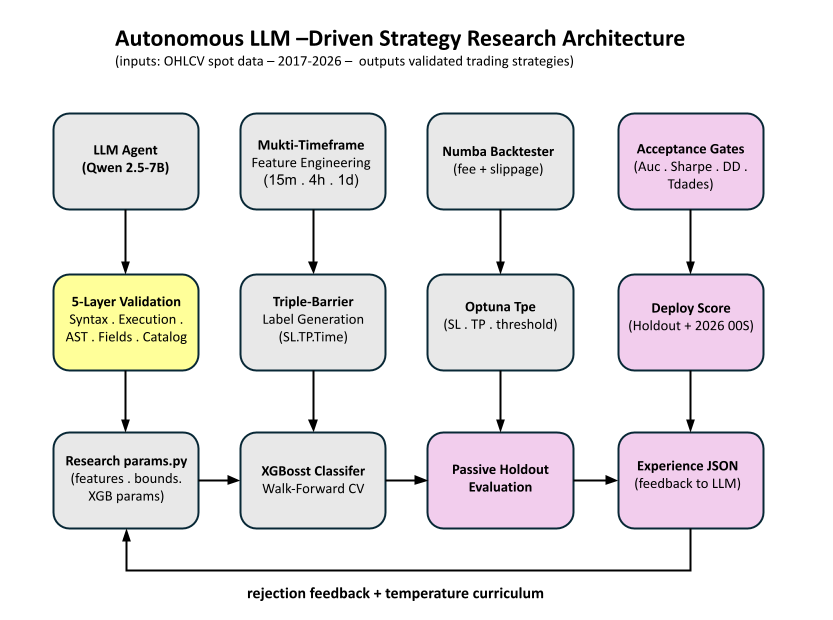
\includegraphics[width=0.85\textwidth]{figures/fig01_architecture_improved.png}
\caption{Autonomous strategy research architecture incorporating LLM-based proposal generation.\label{fig1}}
\end{figure}

\subsection{Feature catalog and temporal-ordering constraints}\label{feature-catalog-and-temporal-ordering-constraints}

All features are computed from OHLCV data at 15-minute, 4-hour, and daily timeframes. The catalog includes technical indicators (RSI, MACD, Bollinger Bands, ADX, ATR, Stochastic RSI, EMA differences), volatility measures, and lagged returns. Every feature is normalized by price or bounded to the current bar, and higher-timeframe indicators are merged into the 15-minute bars only after the corresponding candle has closed. The merge module shifts each higher-timeframe timestamp from its open time to its close time and then uses a backward-looking as-of merge; a daily value observed on day \(t\) therefore first becomes available to the 15-minute model at the close of day \(t\). The validator parses the generated code into an AST and rejects any strategy that references absolute prices after the decision point or that accesses data outside the current bar. These precautions are consistent with standard defenses against leakage in data mining \citep{kaufman_2012} and backtest overfitting \citep{bailey_2017}, and with L\'{o}pez de Prado's \citep{prado_2018} emphasis on purging and embargo in financial cross-validation: observations that overlap a test period due to long investment horizons, or strongly autocorrelated returns, must be excluded from training and from immediate post-test retraining. Our one-bar look-ahead lag for higher-timeframe merges and the AST-based price-reference check implement these principles in code. We treat this temporal-integrity layer as a design invariant; it is enforced in code review and verified by the out-of-sample stability reported in the results.

\subsection{Training and backtesting engine}\label{training-and-backtesting-engine}

Labels are generated with a triple-barrier method \citep{prado_2018}: each trade has a profit-taking barrier, a stop-loss barrier, and a vertical time barrier. An XGBoost classifier \citep{chen_2016} is trained on the training set and predictions are converted into signals. The backtester simulates trades using Numba-accelerated code. Costs are modeled as a 0.20 \% round-trip fee plus 0.10 \% slippage on entry, following the transaction-cost framework used in optimal execution literature \citep{almgren_2001}. Stop-loss and take-profit exits are executed at the triggered level without additional slippage in the baseline configuration; Section 4.5 reports a stress-test that adds up to 0.30 \% symmetric slippage on all exits.

All Sharpe ratios reported by the engine and in the statistical audit are computed from daily equity changes and annualized with \(\sqrt{365}\), the standard convention for cryptocurrency markets. This convention is used consistently across validation, holdout, and the secondary selection holdout periods.

An optional volatility kill-switch (\texttt{atr\_kill}) zeros model probabilities when the 15-minute ATR exceeds a rolling multiple, preventing entries during extreme volatility spikes. The ATR and ADX indicators used for volatility and trend-strength filtering follow the original definitions of Wilder \citep{wilder_1978}. In the selected production candidate (S11 iter 1077), the kill-switch was configured at 3.0 rolling standard deviations. Candidate acceptance also requires a maximum drawdown below -15 \%.

To mitigate overfitting, we use a nested temporal split:

\begin{itemize}
\item
  \textbf{Training}: oldest 60 \% of the in-sample window.
\item
  \textbf{Validation}: next 20 \%, used for early stopping and Optuna.
\item
  \textbf{Holdout}: most recent 20 \%, never seen by Optuna.
\end{itemize}

For Season 12, the split was extended to 2017--2020 training, 2021--2023 validation, and 2024--2025 holdout.

\subsubsection{Walk-forward cross-validation}\label{walk-forward}

Inside the training window, XGBoost hyper-parameter search and the reported cross-validation AUC use scikit-learn's \texttt{TimeSeriesSplit} with three and five folds respectively. Each fold is a contiguous block: fold \(t\) is trained on all observations up to a split point and tested on the immediately following block. This preserves temporal ordering but does not apply explicit purging or embargo between folds; because labels are generated with a triple-barrier that closes trades at a fixed horizon or barrier, the overlap between adjacent training and test folds is limited. The final model is retrained on the full in-sample window after hyper-parameter selection, and only the passive holdout and the secondary selection holdout are used for deploy scoring.

\subsection{LLM agent and prompt engineering}\label{llm-agent-and-prompt-engineering}

The LLM agent is a local Qwen2.5-7B-Instruct model served via llama.cpp. The choice of a 7B-parameter model is deliberate: it is small enough to run locally on consumer-grade GPUs via llama.cpp, which keeps the research loop private (no strategy code or market data is sent to external APIs) and eliminates per-token API costs across tens of thousands of iterations. Despite its size, the model generates syntactically valid Python strategy proposals in the constrained JSON schema used by the pipeline.

Across Season 11, the five-layer validation and scoring infrastructure rejected 94.4\% of the 3,797 candidates: 18.5\% failed code-validation (syntax, execution, AST future-leak, or feature-catalog compliance), 9.1\% were duplicate parameter configurations, 18.8\% converged to a previously discovered Optuna optimum, and 42.7\% passed all code and optimization layers but failed the performance gates (AUC, validation Sharpe, holdout Sharpe, or drawdown). Only 5.6\% were accepted. These rates indicate that the bottleneck is not the LLM's proposal quality per se, but the multi-layer validation and scoring layers that filter out unsound candidates.

The prompt contains:

\begin{itemize}
\item
  The season objective (e.g., ``improve holdout Sharpe on BTC'').
\item
  A summary of the previous season's accepted strategies and common failure modes.
\item
  The feature catalog with exact function signatures.
\item
  A JSON schema for the strategy proposal.
\item
  Examples of valid and invalid code patterns.
\end{itemize}

The agent keeps a memory of recent failures to avoid repetitive proposals. After each season, a human-in-the-loop review (typically 15--30 minutes) updates the season objective and acceptance gates based on the distribution of accepted strategies. This is the primary point of human supervision; within a season, the loop runs without human approval of individual candidates. This mixed-initiative design follows the principles of Horvitz \citep{horvitz_1999} and Amershi et al. \citep{amershi_2019}: the system performs the bulk of routine experimentation and surfaces structured results, while the human retains control over high-level goals and value alignment. The criteria used at each major transition are documented in Supplementary Table~S2.

\subsubsection{Governance and accountability}\label{governance-and-accountability}

Although the loop inside a season is autonomous, several mechanisms constrain the scope of autonomous decisions and allocate accountability.

\textbf{Prompt and schema constraints.} The LLM cannot propose arbitrary code. It must emit a JSON object with fixed fields (\texttt{features}, \texttt{entry\_logic}, \texttt{sl\_pct}, \texttt{tp\_pct}, \texttt{threshold}, \texttt{adx\_min}, \texttt{atr\_kill\_threshold}, \texttt{xgb\_params}) and use only functions from the leakage-free feature catalog. The prompt includes the season objective, a summary of the last 10--20 rejected proposals, and three in-context examples of valid and invalid code patterns. The temperature is initialized at 0.7 and annealed downward when the acceptance rate stalls, reducing exploration once the search has found a productive region.

\textbf{Season-transition review protocol.} At each transition the human reviewer inspects: (i) the distribution of accepted strategies by AUC, Sharpe, and drawdown; (ii) the most common rejection reasons; (iii) the feature-importance patterns of accepted models; and (iv) any evidence of objective drift (e.g., falling validation Sharpe despite rising holdout Sharpe). Based on this, the reviewer updates the season objective, adjusts one or two acceptance bounds, and reweights the composite score. The reviewer records the rationale in \texttt{season\_notes.md}, which becomes part of the audit trail.

\textbf{Accountability allocation.} We adopt a simple RACI-style model for the offline research phase:

\begin{itemize}
\item
  \textbf{Responsible (autonomous agent):} proposing candidates, running backtests, and logging results.
\item
  \textbf{Accountable (human researcher):} setting season objectives, acceptance gates, and scoring weights; interpreting results; and deciding whether a candidate is promoted to further study.
\item
  \textbf{Consulted (code validator, statistical audit):} enforcing hard constraints and flagging suspicious patterns.
\item
  \textbf{Informed (future deployment system):} receiving the selected candidate and parameters, but not involved in research decisions.
\end{itemize}

This model applies to the offline research pipeline only. A subsequent live system would require a separate governance layer with real-time monitoring, circuit breakers, and compliance sign-off that are outside the scope of this paper.

\subsection{Acceptance gates and composite score}\label{acceptance-gates-and-composite-score}

A strategy is accepted only if it satisfies all of the following configurable gates, which changed across seasons:

\begin{itemize}
\item
  Cross-validation AUC above a season-specific threshold (typically $\geq$ 0.52--0.55).
\item
  Sharpe ratio on the validation window above a season-specific threshold (typically $\geq$ 0.5--1.0).
\item
  Sharpe ratio on the passive-holdout window above a season-specific threshold (typically $\geq$ 0.0--0.5).
\item
  Maximum drawdown within the backtest objective bounds (the objective function rejects configurations with excessive drawdown).
\item
  At least a minimum number of trades in the validation window.
\item
  All code-validation layers passed.
\end{itemize}

Strategies are ranked by a composite score that combines the validation Sharpe ratio, the passive-holdout Sharpe ratio, the holdout return, the maximum drawdown, and the cross-validation AUC. Formally, the ranking objective can be written as:

\[S = w_1 \cdot \text{Sharpe}_{\text{val}} + w_2 \cdot \text{Sharpe}_{\text{hold}} + w_3 \cdot \text{Ret}_{\text{oos}} - w_4 \cdot |\text{DD}_{\text{max}}| - w_5 \cdot |\text{AUC}_{\text{cv}} - 0.5|\]

where the weights \(w_i\) were adjusted across seasons. In Seasons 9--12, the weights emphasized holdout Sharpe and drawdown control; strategies with negative holdout Sharpe or validation-holdout decay were heavily penalized. Inside the Bayesian optimizer, the objective function changed from maximizing the minimum validation Sharpe across sub-windows (score mode) to maximizing the average holdout return (profit mode), with hard constraints on drawdown and trade count.

\subsection{Deployment score and model selection}\label{deployment-score-and-model-selection}

For deployment selection, we use a deploy score that averages the passive-holdout Sharpe and the Sharpe on the secondary selection holdout (January--March 2026 for S11):

\[\text{Deploy\_score} = \frac{\text{Sharpe}_{\text{hold}} + \text{Sharpe}_{\text{2026}}}{2}\]

Because the deploy score includes \(\text{Sharpe}_{\text{2026}}\), the 2026 period works as a \textbf{secondary selection holdout}: it was used to choose the production candidate from the 30 top holdout candidates that were re-evaluated for deployment from Season 11. It is therefore not an independent prospective test and should be treated only as a noisy post-selection observation. The selected candidate, S11 iter 1077, had the highest deploy score among these 30 re-evaluated candidates; that score is driven primarily by the passive-holdout Sharpe because the 2026 window contains only four trades and its Sharpe is extremely noisy.

The selected candidate's passive-holdout Sharpe (2.87 on active trading days) comes from a population of 212 accepted strategies in Season 11, so it is also subject to selection bias. Under the simplifying assumption that the 212 accepted holdout Sharpes are i.i.d.~normal with the observed mean (1.37) and standard deviation (0.61), the expected maximum among 212 draws is approximately 3.06 (95 \% interval: 2.66--3.62), and the observed maximum active-day holdout Sharpe of 2.87 lies within the range expected from pure selection; however, the positive mean of the accepted strategies (1.37) indicates that the accepted population as a whole has positive holdout performance. This selection-bias calculation follows the Extreme Value Theory framework developed by \citep{bailey_2014} to estimate performance inflation under multiple testing.

The Q1 2026 Sharpe is based on only four trades and is consequently very noisy; it should not be interpreted as precise evidence of live edge, nor used to rank the candidate against other candidates. We report it as a preliminary post-selection observation rather than as an independent out-of-sample result.

\subsection{Experimental configuration and computational budget}\label{experimental-configuration}

Table~\ref{tab:case-study-strategies} summarizes the two strategies analyzed in detail. Table~\ref{tab:season-evolution} reports how the search evolved across seasons. The full feature catalog is provided in Supplementary Table~S1, and the inter-season design decisions are documented in Supplementary Table~S2.


\begin{longtable}[]{@{}
  >{\raggedright\arraybackslash}p{(\columnwidth - 4\tabcolsep) * \real{0.3333}}
  >{\raggedright\arraybackslash}p{(\columnwidth - 4\tabcolsep) * \real{0.3333}}
  >{\raggedright\arraybackslash}p{(\columnwidth - 4\tabcolsep) * \real{0.3333}}@{}}
\caption{Case-study strategies}\label{tab:case-study-strategies}\\
\toprule\noalign{}
\begin{minipage}[b]{\linewidth}\raggedright
Feature
\end{minipage} & \begin{minipage}[b]{\linewidth}\raggedright
S11 iter 1077 (production)
\end{minipage} & \begin{minipage}[b]{\linewidth}\raggedright
S12 iter 5502 (BTC replication)
\end{minipage} \\
\midrule\noalign{}
\endhead
\bottomrule\noalign{}
\endlastfoot
Asset & BNB/USDT & BTC/USDT \\
Training period & 2022--2023 & 2017--2020 \\
Validation period & 2022--2024 (walk-forward) & 2021--2023 \\
Holdout period & 2025 & 2024--2025 \\
Secondary selection holdout & Jan--Mar 2026 & --- \\
Validation AUC & 0.5721 & 0.5321 \\
Validation Sharpe (active-day) & 1.69 & 1.39 \\
Holdout Sharpe (active-day) & 2.87 & 1.15 \\
Calendar-time holdout Sharpe & 2.34 (2025) & 1.00 (2024--2025) \\
Total return & 58.2 \% (2022--2026, simple sum) & 44.0 \% (2021--2025, simple sum) \\
Holdout return (2024--2025) & --- & 27.7 \% (compounded) \\
Maximum drawdown & -6.74 \% & -8.1 \% \\
Average win rate & 65.9--91.7 \% & 90.9 \% \\
Number of trades & 161 (2022--2026) & 38 (2021--2025) \\
Stop-loss / Take-profit & 7.8 \% / 7.1 \% & 9.7 \% / 9.1 \% \\
Probability threshold & 0.857 & 0.890 \\
Regime filter & ADX $\geq$ 22, ATR kill 3$\sigma$ & ADX implicit in features \\
Modeled costs & 0.20 \% fee + 0.10 \% slippage & 0.20 \% fee + 0.10 \% slippage \\
\end{longtable}

\emph{Note: S11 metrics are produced by \texttt{deployment/evaluate\_models.py} with independent yearly backtests (initial capital EUR~500, \texttt{max\_pos=5}, ATR kill 3.0). The holdout year (2025) was never used during hyper-parameter optimization; the Jan--Mar 2026 period was used to select the production model from 30 re-evaluated candidates and is therefore a noisy post-selection observation (four trades), not an independent prospective test. Validation and holdout Sharpe ratios labeled `active-day' are computed from daily equity changes on days with at least one closed position and annualized with $\sqrt{365}$; the `Calendar-time holdout Sharpe' is computed from the full daily equity curve including inactive days and is the more conservative headline metric.}

The experiments were run on a local workstation with a consumer GPU serving the Qwen2.5-7B-Instruct model via llama.cpp. We did not log exact wall-clock time per iteration, but the full study (34,333 iterations across twelve seasons) required about 6--8 weeks of continuous execution, including restarts after memory-related crashes in early seasons. The LLM inference and Optuna optimization together consumed an estimated 500--800 kWh. Per-iteration latency varied from seconds (for strategies rejected at the code-validation layer) to several minutes (for strategies that ran the full Optuna loop). Future work will add instrumentation to record precise GPU hours and energy consumption.

\subsection{Reproducibility protocol}\label{reproducibility-protocol}

To enable independent replication, we fixed the software environment, random seeds, data sources, and execution flow described below. All code, experiment logs, and generated artifacts are available in the repository associated with this submission.

\textbf{Persistent archive.} All code, experiment logs, and generated artifacts are publicly available at \url{https://github.com/pesobreiro/algo-autoresearch-paper} (MIT license) and are permanently archived at Zenodo (DOI: \url{https://doi.org/10.5281/zenodo.21160587}).

\textbf{Software environment.} The pipeline was executed under Python 3.13.11 with the following core package versions: pandas 3.0.1, NumPy 2.4.3, Numba 0.65.1, XGBoost 3.3.0, scikit-learn 1.9.0, Optuna 4.9.0, Joblib 1.5.3, PyArrow 12.0 or later, and llama.cpp serving Qwen2.5-7B-Instruct (quantized GGUF, Q4\_K\_M). The multi-timeframe feature-merge module is imported from \texttt{features.technical} (commit hash recorded in \texttt{requirements.txt}). The full dependency list is in \texttt{requirements.txt}. We recommend creating a dedicated virtual environment and installing the pinned versions; newer versions may alter random number generation or sampler behavior and are not guaranteed to reproduce the exact numeric results reported here.

\textbf{Random seeds.} Determinism was enforced at three points: (i) the XGBoost classifier uses \texttt{random\_state=42}; (ii) Optuna's TPE sampler is initialized with \texttt{seed=42} and \texttt{n\_startup\_trials=20} for the SL/TP/threshold study (and \texttt{n\_startup\_trials=max(5,\ n\_trials\ //\ 4)} when XGBoost hyper-parameters are also tuned); (iii) scikit-learn's \texttt{TimeSeriesSplit} is used for walk-forward cross-validation. Because some operations rely on Numba JIT compilation and BLAS threading, byte-identical reproduction across operating systems is not guaranteed; the statistical conclusions, however, are robust to the residual non-determinism.

\textbf{Hardware.} The main experiments ran on a Linux workstation with an NVIDIA GeForce RTX 2060 (6 GB) and an x86\_64 CPU. The LLM server (\texttt{llama-server}) offloaded 32 layers to the GPU; the remaining CPU layers introduced per-token latency but no change to the generated distribution beyond temperature effects. CPU-only execution is possible but substantially slower.

\textbf{Data.} OHLCV bars at 15-minute, 4-hour, and daily resolutions were downloaded from the Binance public API and stored as Parquet files in a dedicated data directory (\texttt{\textasciitilde{}/crypto\_data}). The raw data are publicly available; the ticker mappings are \texttt{bnb\_15m\_usdt\_binance}, \texttt{bnb\_4h\_usdt\_binance}, \texttt{bnb\_1d\_usdt\_binance} for BNB/USDT and \texttt{btc\_15m\_usdt\_binance}, etc., for BTC/USDT. We used the closing prices from the daily series to compute the buy-and-hold benchmarks. A \texttt{download\_data.py} helper script in the repository performs the exact Binance API calls used in this study and records the date ranges of each file.

\textbf{Repository structure.} The repository contains:

\begin{itemize}
\tightlist
\item
  \texttt{autoresearch/} --- LLM client, validator, tracker, and runner.
\item
  \texttt{pipeline/} --- label generation, XGBoost training, Optuna backtest, feature catalog, and \texttt{research\_params.py} (the single file the LLM is allowed to rewrite each iteration).
\item
  \texttt{experiments\_s\{season\}/} --- one JSON file per iteration with metrics, parameters, and status.
\item
  \texttt{best\_models/season\_\{season\}/} --- accepted model artifacts.
\item
  \texttt{deployment/} --- scripts to re-run the selected case studies and produce annual performance tables and benchmark comparisons.
\end{itemize}

\textbf{Execution flow.} A single season is launched with \texttt{python\ main.py} after copying \texttt{config.yaml.example} to \texttt{config.yaml} and starting the local LLM server. The runner executes the loop described in Section~3.1: proposal, validation, training, Optuna optimization, and holdout evaluation. The configuration file specifies the ticker, exchange, data directory, season identifier, and acceptance minima; the exact feature sets, indicator parameters, SL/TP/threshold ranges, and XGBoost hyper-parameters are written by the LLM into \texttt{pipeline/research\_params.py} each iteration. For post-hoc verification, the deployment scripts \texttt{deployment/evaluate\_models.py} and \texttt{deployment/backtest\_deploy.py} replay the selected iterations using the saved model and parameters, without calling the LLM.

\textbf{Reproduction checklist.} To replicate the two case studies reported in Section~4: (1) install the pinned environment; (2) download the Binance OHLCV data for BNB/USDT and BTC/USDT at the three timeframes; (3) start the LLM server with the Qwen2.5-7B-Instruct GGUF model; (4) run \texttt{python\ main.py} with the appropriate season number; (5) for the selected iterations, run the deployment scripts with the parameters recorded in \texttt{best\_models/season\_\{N\}/iter\_\{XXXX\}/meta.json}. Because the search is expensive, a partial reproduction can focus on rerunning the saved case studies, which is computationally cheap and fully deterministic given the saved model and parameters.

\section{Results}\label{results}

\subsection{Search convergence across experimental seasons}\label{search-convergence-across-experimental-seasons}

\begin{figure}[H]
\centering
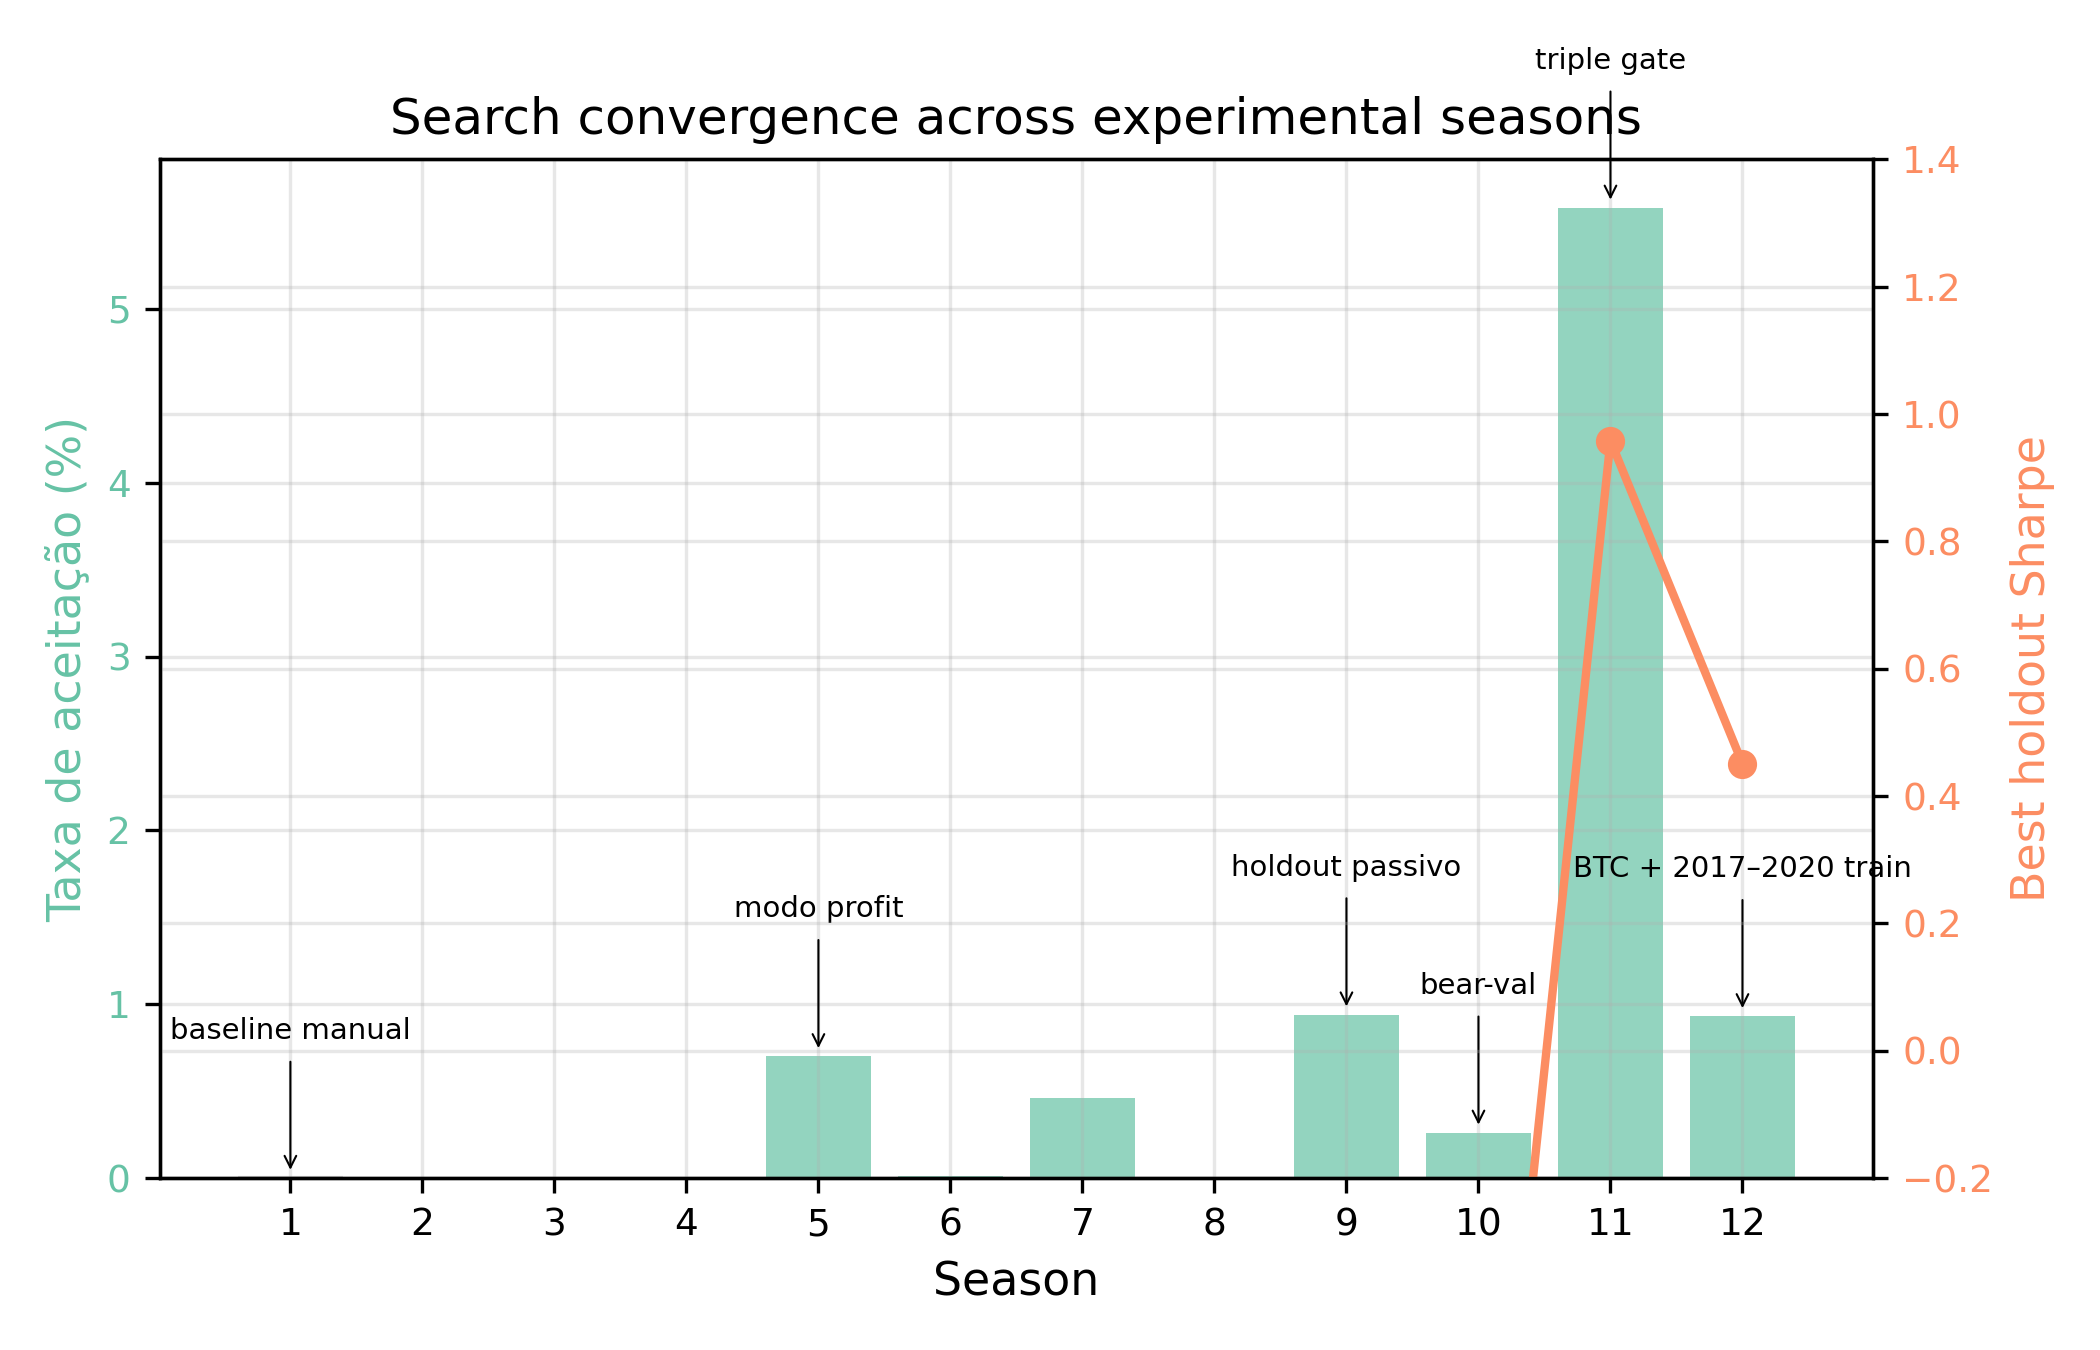
\includegraphics[width=0.85\textwidth]{figures/fig02_search_convergence.png}
\caption{Search convergence across experimental seasons (acceptance rate and best holdout Sharpe).\label{fig2}}
\end{figure}


\begin{longtable}[]{@{}
  >{\raggedright\arraybackslash}p{(\columnwidth - 12\tabcolsep) * \real{0.1111}}
  >{\raggedleft\arraybackslash}p{(\columnwidth - 12\tabcolsep) * \real{0.1481}}
  >{\raggedleft\arraybackslash}p{(\columnwidth - 12\tabcolsep) * \real{0.1481}}
  >{\raggedleft\arraybackslash}p{(\columnwidth - 12\tabcolsep) * \real{0.1481}}
  >{\raggedleft\arraybackslash}p{(\columnwidth - 12\tabcolsep) * \real{0.1481}}
  >{\raggedleft\arraybackslash}p{(\columnwidth - 12\tabcolsep) * \real{0.1481}}
  >{\raggedleft\arraybackslash}p{(\columnwidth - 12\tabcolsep) * \real{0.1481}}@{}}
\caption{Evolution of acceptance rate and best holdout Sharpe by season}\\
\toprule\noalign{}
\begin{minipage}[b]{\linewidth}\raggedright
Season
\end{minipage} & \begin{minipage}[b]{\linewidth}\raggedleft
Asset
\end{minipage} & \begin{minipage}[b]{\linewidth}\raggedleft
Iterations
\end{minipage} & \begin{minipage}[b]{\linewidth}\raggedleft
Accepted
\end{minipage} & \begin{minipage}[b]{\linewidth}\raggedleft
Acceptance rate (\%)
\end{minipage} & \begin{minipage}[b]{\linewidth}\raggedleft
Best holdout Sharpe
\end{minipage} & \begin{minipage}[b]{\linewidth}\raggedleft
Iteration of best holdout
\end{minipage} \\
\midrule\noalign{}
\endhead
\bottomrule\noalign{}
\endlastfoot
1 & BNB & 32 & 0 & 0.00 & --- & --- \\
2 & BNB & 20 & 0 & 0.00 & --- & --- \\
3 & BNB & 367 & 0 & 0.00 & --- & --- \\
4 & BNB & 2,903 & 0 & 0.00 & --- & --- \\
5 & BNB & 1,419 & 10 & 0.70 & --- & --- \\
6 & BNB & 12,864 & 1 & 0.01 & --- & --- \\
7 & ETH & 1,096 & 5 & 0.46 & --- & --- \\
8 & BTC & 176 & 0 & 0.00 & --- & --- \\
9 & BNB & 534 & 5 & 0.94 & 1.00 & 178 \\
10 & BNB & 1,168 & 3 & 0.26 & 2.41 & 326 \\
11 & BNB & 3,797 & 212 & 5.58 & 2.95 & 1,133 \\
12 & BTC & 9,957 & 93 & 0.93 & 1.23 & 1,736 \\
\label{tab:season-evolution}
\end{longtable}

\emph{Note: Season 1 was a manual initialization/baseline phase before the automated loop started at Season 2. Scores in S5--S7 used a different scale from S9--S12; the table therefore reports holdout Sharpe as the cross-season comparable metric.}

Figure~2 shows the acceptance rate and the best holdout Sharpe ratio per season. Season 1 was the manual initialization baseline (32 iterations, score 0.5607, no formal acceptance gates); the automated loop started at Season 2. The early automated seasons (S2--S4) produced no accepted strategies because the acceptance gates were too loose or the search space too unconstrained. Season 5 introduced a profit-mode objective and achieved the first acceptances (0.70 \%). Season 6 introduced stricter criteria, dropping the acceptance rate to 0.01 \% (1 in 12,864). Seasons 9--12 improve steadily in holdout Sharpe, driven by three changes: passive holdout (S9), bear-market validation (S10), and the triple-gate protocol (S11). Season 12 extended the training window back to 2017 and switched to BTC, a test of cross-asset generalization.

The acceptance rate reached its peak of 5.58 \% in Season 11, but this reflects a richer proposal distribution, not weaker gates: the average composite score fell from 2.03 in S9 to 1.09 in S11 because the scoring weights were renormalized when the acceptance gates tightened (S9 allowed only five strategies with high validation Sharpe but negative average holdout Sharpe; S11 demanded positive holdout Sharpe and lower drawdown, which compressed the score scale). The best holdout Sharpe rose from 1.00 to 2.95 over the same period, so quality improved even as the raw score range shifted.

\subsection{Production model performance}\label{production-model-performance}

The selected production candidate, S11 iter 1077, traded BNB/USDT from 2022 to March 2026. Figure~3 shows the equity curve. Table~\ref{tab:s11-annual-performance} gives the annual performance. The candidate produced positive returns in 2022--2025 on the passive-holdout and validation windows. The 2026 window was used only for deployment selection and is reported as a post-selection observation. The maximum drawdown was -6.74 \%, well below the -15 \% gate. Table~\ref{tab:s11-benchmark} compares these returns with a passive buy-and-hold investment in BNB/USDT over the same period.

\begin{figure}[H]
\centering
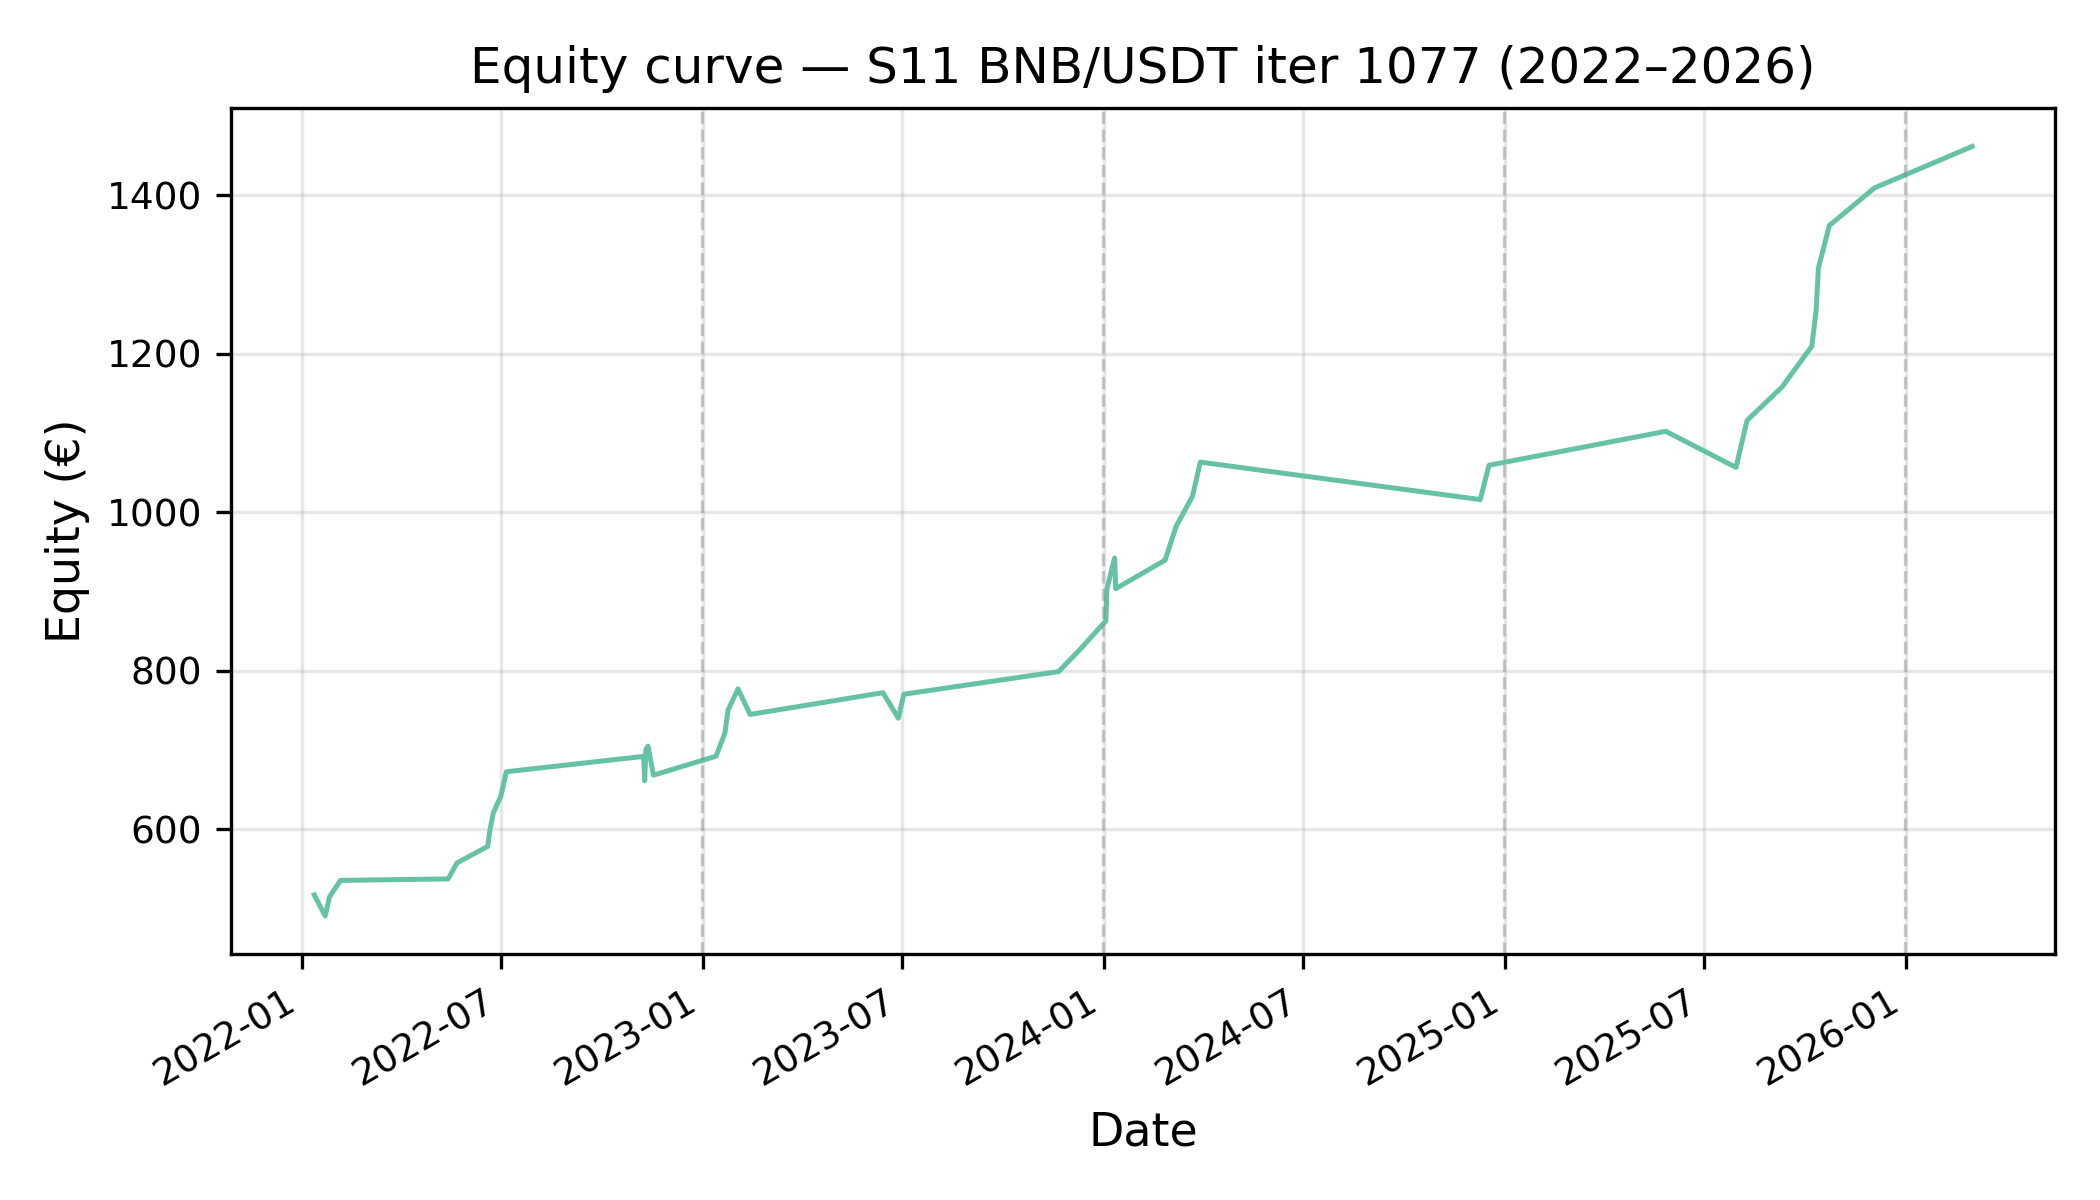
\includegraphics[width=0.85\textwidth]{figures/fig03_equity_s11_1077.png}
\caption{Equity curve --- S11 BNB/USDT iter 1077 (2022--2026).\label{fig3}}
\end{figure}

The strategy's AUC of 0.5721 shows only marginal predictive power at the individual-bar level; the economic value comes from combining a calibrated probability threshold, asymmetric risk management (7.8 \% stop-loss vs.~7.1 \% take-profit), and an ADX regime filter \citep{wilder_1978} that avoids weak-trend entries. The wider stop-loss relative to take-profit came from Optuna optimization under the bear-market validation introduced in Season 10: it gives profitable trades room to survive short-term reversals while the high-probability threshold and ADX filter keep entry quality high enough that smaller, more frequent gains offset occasional larger losses.

\textbf{Benchmark comparison.} Table~\ref{tab:s11-benchmark} compares the strategy's annual returns with a passive buy-and-hold investment in BNB/USDT.


\begin{longtable}[]{@{}
  >{\raggedleft\arraybackslash}p{(\columnwidth - 12\tabcolsep) * \real{0.1429}}
  >{\raggedleft\arraybackslash}p{(\columnwidth - 12\tabcolsep) * \real{0.1429}}
  >{\raggedleft\arraybackslash}p{(\columnwidth - 12\tabcolsep) * \real{0.1429}}
  >{\raggedleft\arraybackslash}p{(\columnwidth - 12\tabcolsep) * \real{0.1429}}
  >{\raggedleft\arraybackslash}p{(\columnwidth - 12\tabcolsep) * \real{0.1429}}
  >{\raggedleft\arraybackslash}p{(\columnwidth - 12\tabcolsep) * \real{0.1429}}
  >{\raggedleft\arraybackslash}p{(\columnwidth - 12\tabcolsep) * \real{0.1429}}@{}}
\caption{Annual performance of the selected production candidate (S11 iter 1077, BNB/USDT)}\label{tab:s11-annual-performance}\\
\toprule\noalign{}
\begin{minipage}[b]{\linewidth}\raggedleft
Year
\end{minipage} & \begin{minipage}[b]{\linewidth}\raggedleft
Return (\%)
\end{minipage} & \begin{minipage}[b]{\linewidth}\raggedleft
Sharpe
\end{minipage} & \begin{minipage}[b]{\linewidth}\raggedleft
Sortino
\end{minipage} & \begin{minipage}[b]{\linewidth}\raggedleft
Max DD (\%)
\end{minipage} & \begin{minipage}[b]{\linewidth}\raggedleft
Trades
\end{minipage} & \begin{minipage}[b]{\linewidth}\raggedleft
Win rate (\%)
\end{minipage} \\
\midrule\noalign{}
\endhead
\bottomrule\noalign{}
\endlastfoot
2022 & 16.75 & 1.40 & 0.57 & -6.74 & 82 & 65.9 \\
2023 & 7.80 & 1.05 & 0.26 & -5.86 & 27 & 70.4 \\
2024 & 15.80 & 2.59 & 0.98 & -1.85 & 24 & 91.7 \\
2025 & 15.90 & 2.87 & 1.96 & -1.70 & 24 & 91.7 \\
2026 & 1.94 & (post-selection, 4 trades) & --- & 0.00 & 4 & 75.0 \\
\end{longtable}

\emph{Note: Annual returns are computed from the deployment simulation with independent yearly resets (EUR~500 per year) and modeled costs of 0.20 \% fee + 0.10 \% slippage. Sharpe ratios are computed from daily equity changes on active trading days (days with at least one closed position) and annualized with $\sqrt{365}$; calendar-time Sharpe, which includes all days, is the more conservative headline metric and is reported in Section~4.6. The 2026 figure covers 1 January--31 March and was used in the deployment-selection criterion; it is not an independent prospective test and is based on only four trades.}


\begin{longtable}[]{@{}
  >{\raggedleft\arraybackslash}p{(\columnwidth - 6\tabcolsep) * \real{0.2500}}
  >{\raggedleft\arraybackslash}p{(\columnwidth - 6\tabcolsep) * \real{0.2500}}
  >{\raggedleft\arraybackslash}p{(\columnwidth - 6\tabcolsep) * \real{0.2500}}
  >{\raggedleft\arraybackslash}p{(\columnwidth - 6\tabcolsep) * \real{0.2500}}@{}}
\caption{Benchmark comparison: S11 iter 1077 vs.~BNB/USDT buy-and-hold}\label{tab:s11-benchmark}\\
\toprule\noalign{}
\begin{minipage}[b]{\linewidth}\raggedleft
Year
\end{minipage} & \begin{minipage}[b]{\linewidth}\raggedleft
S11 iter 1077 (\%)
\end{minipage} & \begin{minipage}[b]{\linewidth}\raggedleft
BNB/USDT buy-and-hold (\%)
\end{minipage} & \begin{minipage}[b]{\linewidth}\raggedleft
Difference (\%)
\end{minipage} \\
\midrule\noalign{}
\endhead
\bottomrule\noalign{}
\endlastfoot
2022 & 16.75 & -53.29 & +70.04 \\
2023 & 7.80 & 27.58 & -19.78 \\
2024 & 15.80 & 124.02 & -108.22 \\
2025 & 15.90 & 22.10 & -6.20 \\
2026 (Jan--Mar) & 1.94 & -29.34 & +31.28 \\
\textbf{Total (2022--Mar 2026)} & \textbf{58.20} & \textbf{17.09} & \textbf{+41.11} \\
\textbf{Max drawdown} & \textbf{-6.74} & \textbf{-62.90} & \textbf{+56.16} \\
\end{longtable}

\emph{Note: S11 iter 1077 returns are from the deployment simulation (\texttt{evaluate\_models.py}) with modeled costs 0.20 \% fee + 0.10 \% slippage. BNB/USDT buy-and-hold returns are computed from daily close prices downloaded from the Binance public API; they ignore funding, staking, and custody costs. The 2026 buy-and-hold figure covers 1 January--31 March 2026.}

\subsection{Cross-asset generalization}\label{cross-asset-generalization}

To test whether the design works across assets, we ran Season 12 on BTC/USDT with a training window starting in 2017. The selected candidate, S12 iter 5502, passed the validation gates and showed a validation Sharpe of 1.39 and a holdout Sharpe of 1.15, with a 27.7 \% holdout return (2024--2025) and a maximum drawdown of -8.1 \% (Figure~4). Table~\ref{tab:s12-annual-performance} breaks down the annual performance. Returns are positive in every year; the weakest years were 2021 (a late-bull period) and 2024 (a sideways-to-down phase). The lower holdout Sharpe relative to S11 reflects Bitcoin's different volatility regime, but the candidate remained profitable and within risk limits.


\begin{longtable}[]{@{}
  >{\raggedright\arraybackslash}p{(\columnwidth - 12\tabcolsep) * \real{0.0870}}
  >{\raggedleft\arraybackslash}p{(\columnwidth - 12\tabcolsep) * \real{0.1739}}
  >{\raggedleft\arraybackslash}p{(\columnwidth - 12\tabcolsep) * \real{0.1159}}
  >{\raggedleft\arraybackslash}p{(\columnwidth - 12\tabcolsep) * \real{0.1304}}
  >{\raggedleft\arraybackslash}p{(\columnwidth - 12\tabcolsep) * \real{0.1739}}
  >{\raggedleft\arraybackslash}p{(\columnwidth - 12\tabcolsep) * \real{0.1159}}
  >{\raggedleft\arraybackslash}p{(\columnwidth - 12\tabcolsep) * \real{0.2029}}@{}}
\caption{Annual performance of the cross-asset replication (S12 iter 5502, BTC/USDT)}\label{tab:s12-annual-performance}\\
\toprule\noalign{}
\begin{minipage}[b]{\linewidth}\raggedright
Year
\end{minipage} & \begin{minipage}[b]{\linewidth}\raggedleft
Return (\%)
\end{minipage} & \begin{minipage}[b]{\linewidth}\raggedleft
Sharpe
\end{minipage} & \begin{minipage}[b]{\linewidth}\raggedleft
Sortino
\end{minipage} & \begin{minipage}[b]{\linewidth}\raggedleft
Max DD (\%)
\end{minipage} & \begin{minipage}[b]{\linewidth}\raggedleft
Trades
\end{minipage} & \begin{minipage}[b]{\linewidth}\raggedleft
Win rate (\%)
\end{minipage} \\
\midrule\noalign{}
\endhead
\bottomrule\noalign{}
\endlastfoot
2021 & 3.7 & 0.69 & 0.16 & -4.6 & 13 & 69.2 \\
2022 & 12.3 & 1.73 & 1.22 & -1.1 & 20 & 80.0 \\
2023 & 13.3 & 2.22 & 1.57 & -1.0 & 16 & 93.8 \\
2024 & 5.4 & 0.70 & 0.35 & -8.0 & 28 & 60.7 \\
2025 & 9.3 & 1.41 & 0.56 & -3.9 & 22 & 68.2 \\
\end{longtable}

\emph{Note: Annual returns are computed independently (EUR~500 reset at the start of each year) to make years comparable. The 2021--2023 window was used for validation, 2024--2025 for holdout.}

\textbf{Benchmark comparison.} Table~\ref{tab:s12-benchmark} compares the S12 strategy's annual returns with a passive buy-and-hold investment in BTC/USDT. As with the S11 case, the strategy underperforms buy-and-hold in strong bull years (2021, 2023, 2024) but avoids most of the bear-market drawdown and produced positive returns in 2022 and 2025 when the benchmark was negative.


\begin{longtable}[]{@{}
  >{\raggedleft\arraybackslash}p{(\columnwidth - 6\tabcolsep) * \real{0.2500}}
  >{\raggedleft\arraybackslash}p{(\columnwidth - 6\tabcolsep) * \real{0.2500}}
  >{\raggedleft\arraybackslash}p{(\columnwidth - 6\tabcolsep) * \real{0.2500}}
  >{\raggedleft\arraybackslash}p{(\columnwidth - 6\tabcolsep) * \real{0.2500}}@{}}
\caption{Benchmark comparison: S12 iter 5502 vs.~BTC/USDT buy-and-hold}\\
\toprule\noalign{}
\begin{minipage}[b]{\linewidth}\raggedleft
Year
\end{minipage} & \begin{minipage}[b]{\linewidth}\raggedleft
S12 iter 5502 (\%)
\end{minipage} & \begin{minipage}[b]{\linewidth}\raggedleft
BTC/USDT buy-and-hold (\%)
\end{minipage} & \begin{minipage}[b]{\linewidth}\raggedleft
Difference (\%)
\end{minipage} \\
\midrule\noalign{}
\endhead
\bottomrule\noalign{}
\endlastfoot
2021 & 3.7 & 57.57 & -53.87 \\
2022 & 12.3 & -65.34 & +77.64 \\
2023 & 13.3 & 154.46 & -141.16 \\
2024 & 5.4 & 111.81 & -106.41 \\
2025 & 9.3 & -7.34 & +16.64 \\
\textbf{Total (2021--2025)} & \textbf{44.0} & \textbf{198.82} & \textbf{-154.82} \\
\textbf{Max drawdown} & \textbf{-8.0} & \textbf{-77.57} & \textbf{+69.57} \\
\label{tab:s12-benchmark}
\end{longtable}

\emph{Note: S12 iter 5502 returns are from the deployment simulation with modeled costs (0.20 \% fee + 0.10 \% slippage) and independent yearly resets (EUR~500 per year); the Total (2021--2025) figure is the simple sum of the annual returns, not a compounded multi-year return. BTC/USDT buy-and-hold returns are computed from Binance daily close prices and ignore funding and custody costs. Max drawdown for buy-and-hold is the largest peak-to-trough decline over 2021--2025.}

\begin{figure}[H]
\centering
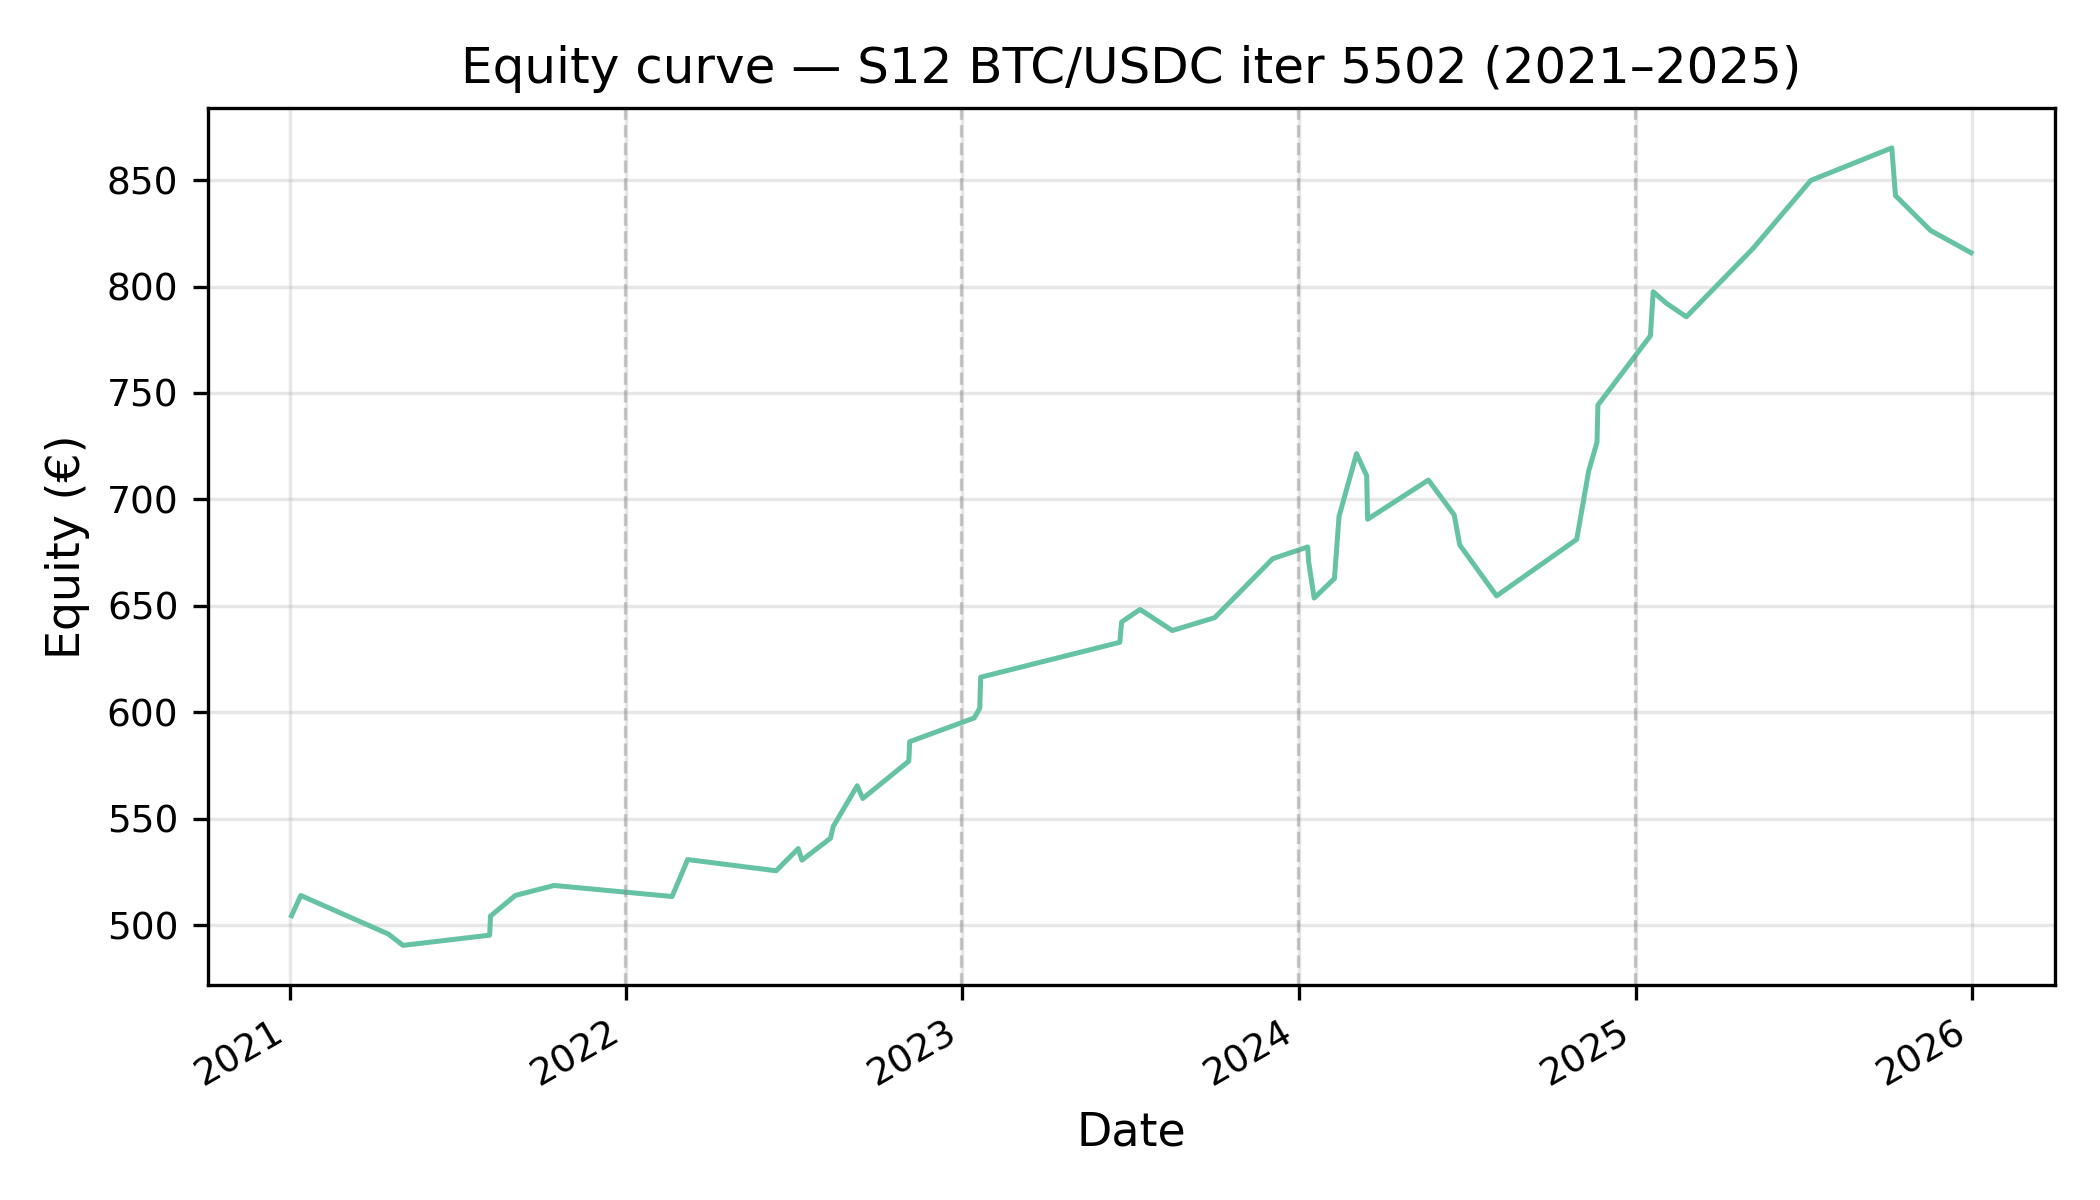
\includegraphics[width=0.85\textwidth]{figures/fig04_equity_s12_5502.png}
\caption{Equity curve --- S12 BTC/USDT iter 5502 (2021--2025).\label{fig4}}
\end{figure}

The lower holdout Sharpe relative to S11 reflects Bitcoin's different volatility regime, but the candidate remained profitable and within risk limits. This indicates that a research system incorporating an LLM agent can adapt its feature selection and risk parameters to a different asset while preserving temporal integrity.

\subsection{Feature importance and parameter sensitivity}\label{feature-importance-and-parameter-sensitivity}

Figure 5 shows the top features for S12 iter 5502. Stochastic RSI and ADX at the daily and 15-minute timeframes dominate, followed by EMA differences and Bollinger Band width. The multi-timeframe pattern matches the findings of \citep{sobreiro_2026} for Bitcoin prediction: short-term momentum and medium-term trend strength carry complementary information. Reference \citep{sobreiro_2026} is by the same first author and shares the OHLCV data source and multi-timeframe feature-engineering approach; we cite it because it documents the same empirical regularity, not as independent validation.

\begin{figure}[H]
\centering
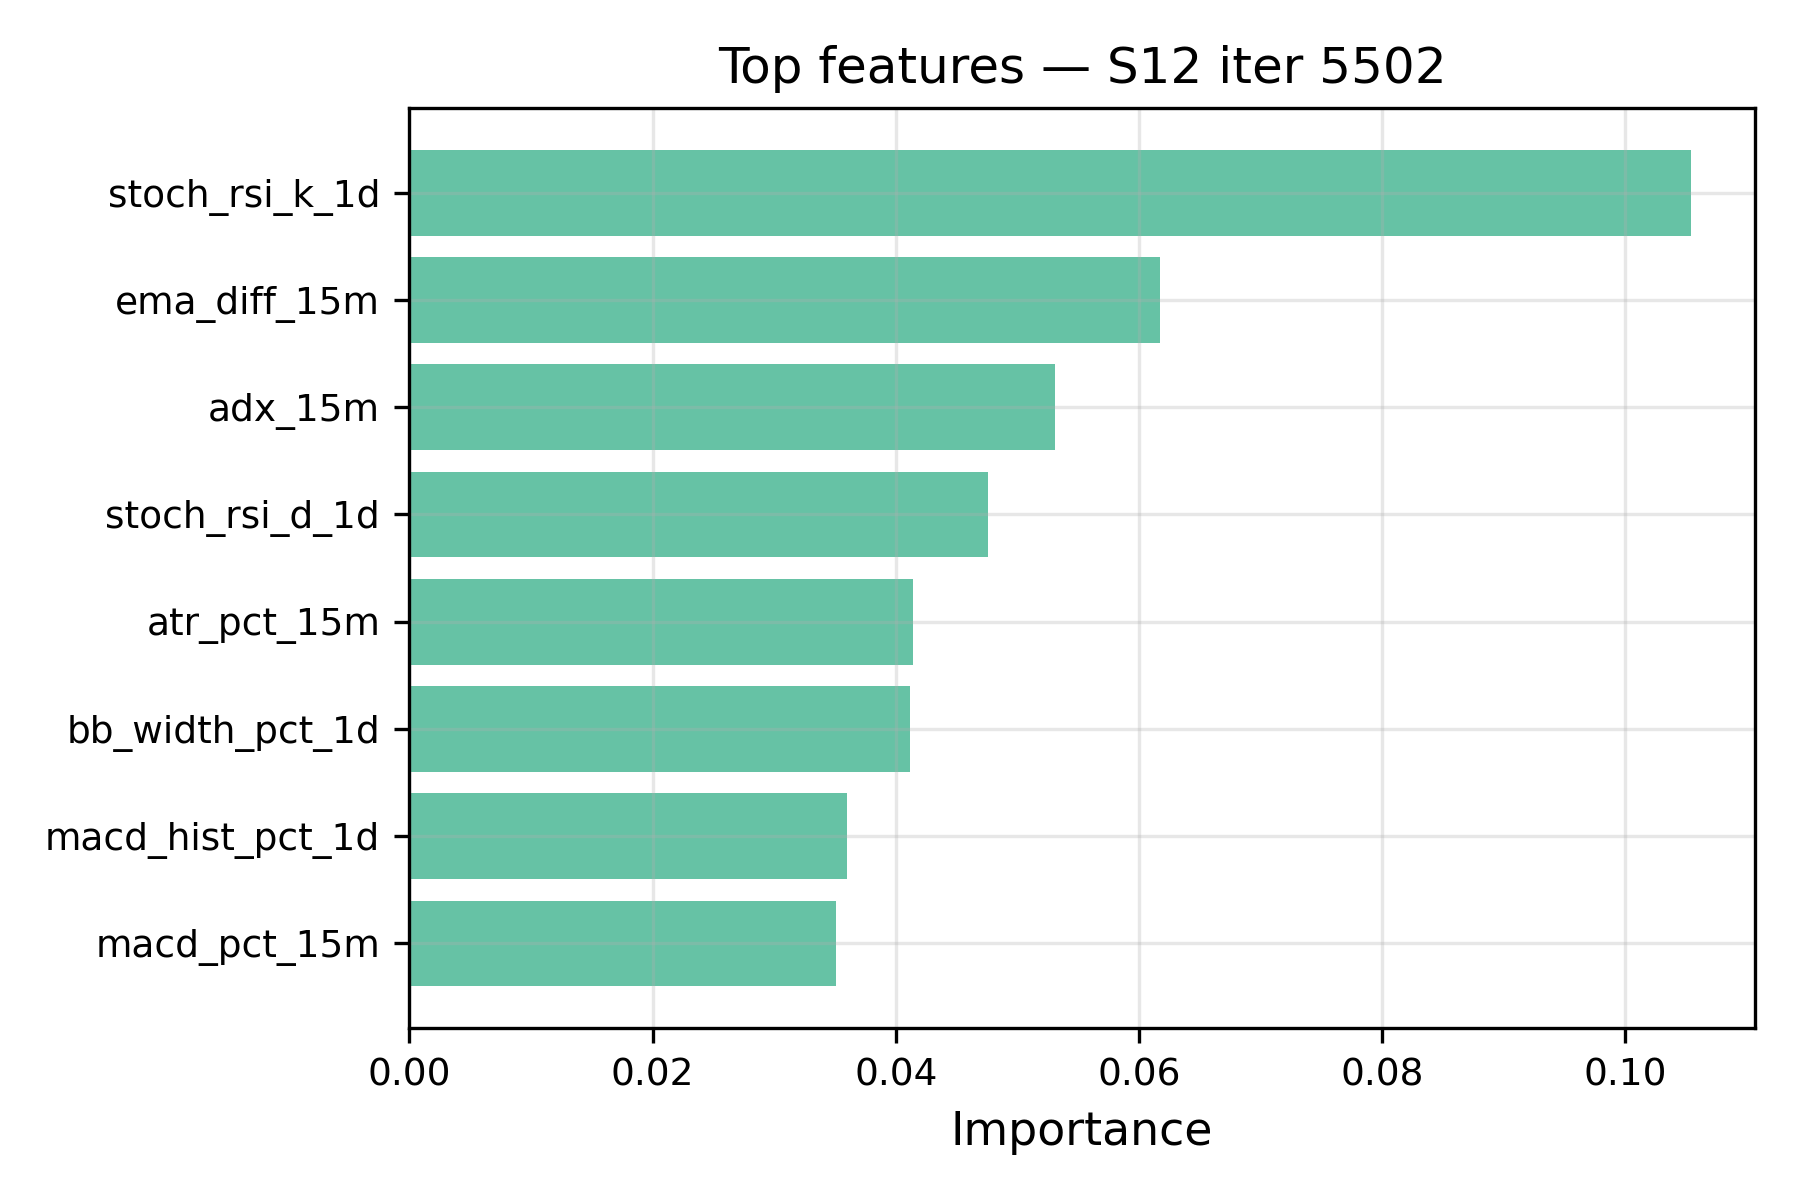
\includegraphics[width=0.85\textwidth]{figures/fig05_feature_importance_s12_5502.png}
\caption{Top features --- S12 iter 5502.\label{fig5}}
\end{figure}

Optuna parameter importance (Figure~6) shows that the probability threshold explains 82--88 \% of the optimization variance across seasons, while stop-loss and take-profit contribute the remainder. This means that trade selection precision matters more than exact exit levels, once the exit range is broadly correct.

\begin{figure}[H]
\centering
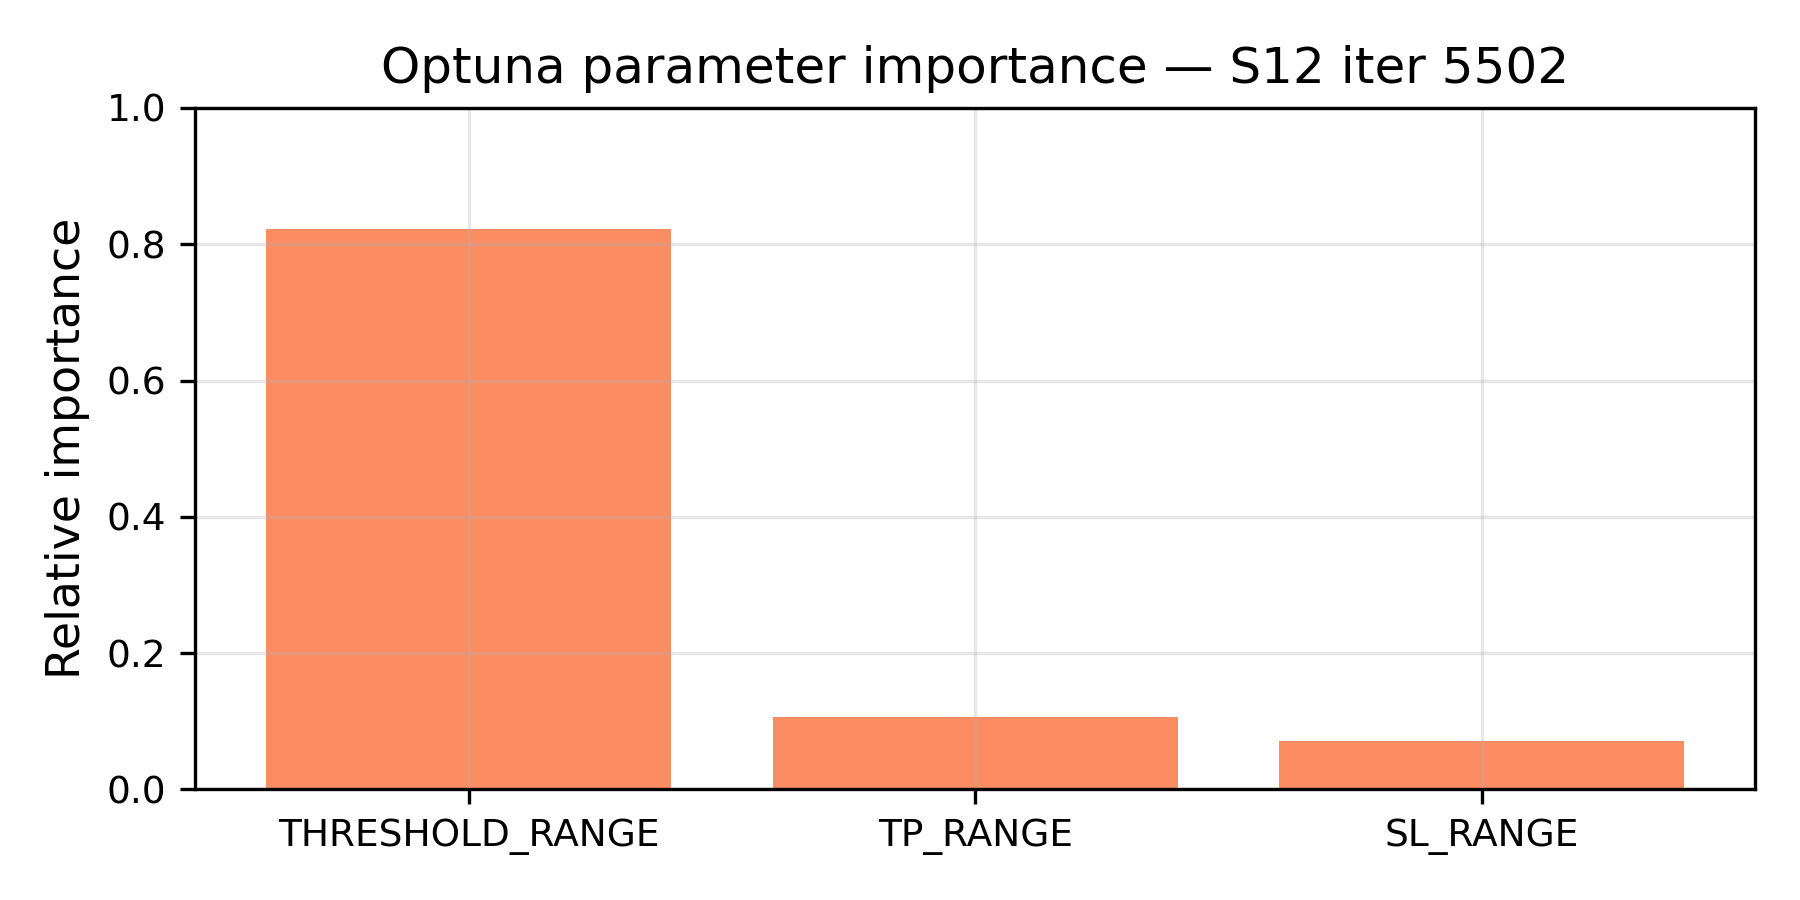
\includegraphics[width=0.85\textwidth]{figures/fig05b_param_importance_s12_5502.png}
\caption{Optuna parameter importance --- S12 iter 5502.\label{fig5b}}
\end{figure}

\subsection{Robustness to transaction costs and market regime}\label{robustness-to-transaction-costs-and-market-regime}

Figure~7 shows the sensitivity of S12 iter 5502 to round-trip transaction costs. Even with costs rising to 1.0 \%, the final equity remains well above the break-even line, so the strategy's edge is not an artifact of unrealistic cost assumptions.

\begin{figure}[H]
\centering
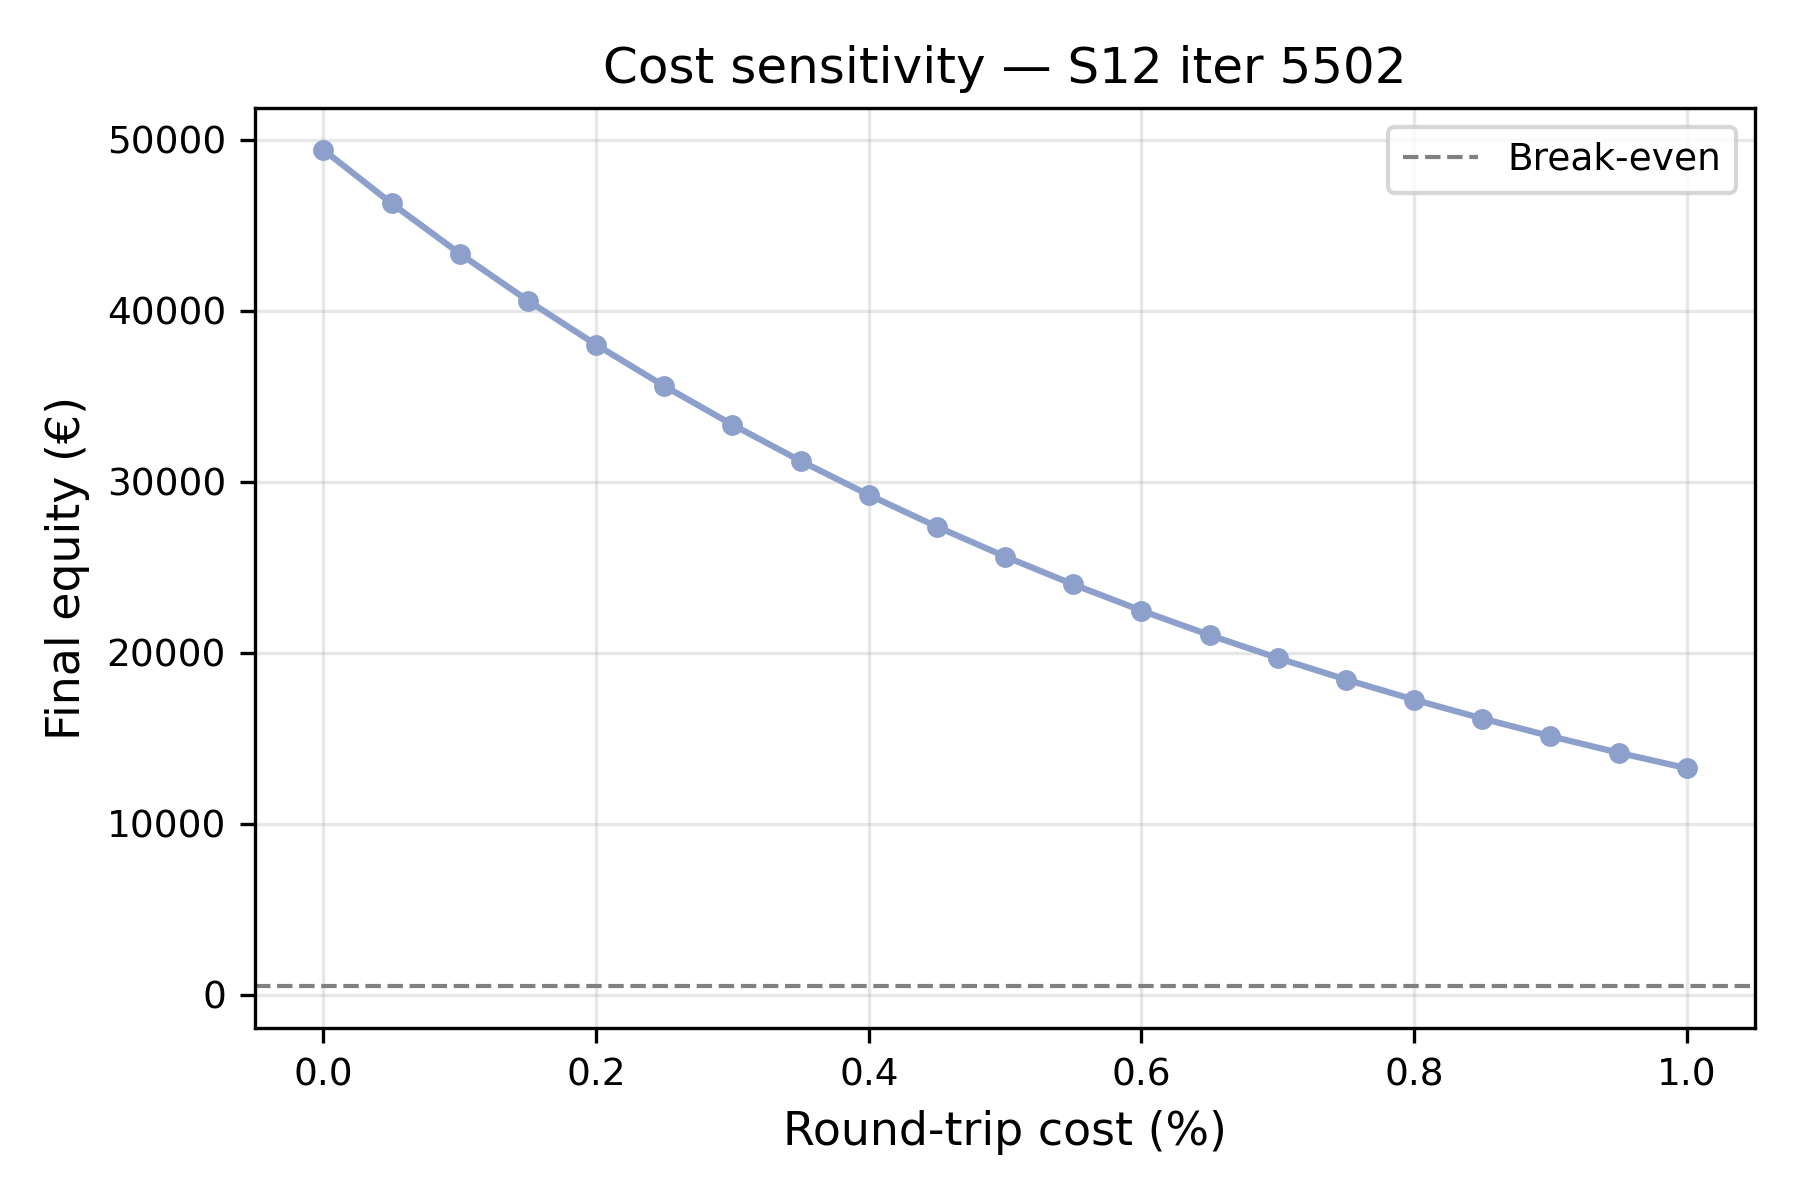
\includegraphics[width=0.85\textwidth]{figures/fig06_cost_sensitivity_s12_5502.png}
\caption{Cost sensitivity --- S12 iter 5502.\label{fig6}}
\end{figure}

\textbf{Exit-slippage stress-test.} The baseline backtest applies 0.10 \% slippage on entry but assumes stop-loss, take-profit, and end-of-period exits execute at the triggered level. Table~\ref{tab:exit-slippage-stress-test} shows the sensitivity of the two case studies to additional symmetric slippage on all exits. Even with an additional 0.30 \% slippage on every exit, both strategies remain profitable on the passive holdout, so the results are not driven by the zero-exit-slippage assumption alone. The S11 case is particularly robust because its wide stop-loss (7.8 \%) and take-profit (7.1 \%) levels mean that small exit slippages are a modest fraction of the expected trade return; the S12 case degrades more quickly because its similarly wide exits are applied to a more volatile asset.

\begin{longtable}[]{@{}
  >{\raggedleft\arraybackslash}p{(\columnwidth - 12\tabcolsep) * \real{0.1429}}
  >{\raggedleft\arraybackslash}p{(\columnwidth - 12\tabcolsep) * \real{0.1429}}
  >{\raggedleft\arraybackslash}p{(\columnwidth - 12\tabcolsep) * \real{0.1429}}
  >{\raggedleft\arraybackslash}p{(\columnwidth - 12\tabcolsep) * \real{0.1429}}
  >{\raggedleft\arraybackslash}p{(\columnwidth - 12\tabcolsep) * \real{0.1429}}
  >{\raggedleft\arraybackslash}p{(\columnwidth - 12\tabcolsep) * \real{0.1429}}
  >{\raggedleft\arraybackslash}p{(\columnwidth - 12\tabcolsep) * \real{0.1429}}@{}}
\caption{Exit-slippage stress-test}\label{tab:exit-slippage-stress-test}\\
\toprule\noalign{}
\begin{minipage}[b]{\linewidth}\raggedleft
Exit slippage (\%)
\end{minipage} & \begin{minipage}[b]{\linewidth}\raggedleft
S11 val Sharpe
\end{minipage} & \begin{minipage}[b]{\linewidth}\raggedleft
S11 holdout Sharpe
\end{minipage} & \begin{minipage}[b]{\linewidth}\raggedleft
S11 total return (\%)
\end{minipage} & \begin{minipage}[b]{\linewidth}\raggedleft
S12 val Sharpe
\end{minipage} & \begin{minipage}[b]{\linewidth}\raggedleft
S12 holdout Sharpe
\end{minipage} & \begin{minipage}[b]{\linewidth}\raggedleft
S12 total return (\%)
\end{minipage} \\
\midrule\noalign{}
\endhead
\bottomrule\noalign{}
\endlastfoot
0.00 & 1.68 & 2.88 & 58.3 & 1.33 & 1.41 & 43.9 \\
0.10 & 1.63 & 2.87 & 56.3 & 1.31 & 1.30 & 40.5 \\
0.20 & 1.60 & 2.85 & 55.2 & 1.28 & 1.28 & 39.4 \\
0.30 & 1.56 & 2.84 & 53.1 & 1.26 & 1.26 & 38.1 \\
\end{longtable}

\emph{Note: Entry slippage is fixed at 0.10 \% and the round-trip fee at 0.20 \%. Exit slippage is applied symmetrically to stop-loss, take-profit, and end-of-period exits. S11 values cover 2022--2026; S12 values cover 2021--2025. Total return is the simple sum of annual returns with independent yearly resets (EUR~500 per year).}

Figure~8 reports mean trade return by ADX regime. The strategy performs best in trending markets (ADX 20--40) and strong-trend markets (ADX \textgreater{} 40), while staying roughly flat in weak-trend/lateral regimes. Table~\ref{tab:adx-regime-trades} reports the trade counts underlying these means; the reliability of the weak-trend estimate is low because few or no trades occur in that bin. This pattern matches the ADX filter \citep{wilder_1978} embedded in the feature set and the broader class of regime-switching models that partition returns by state variables \citep{hamilton_1989}.

\begin{figure}[H]
\centering
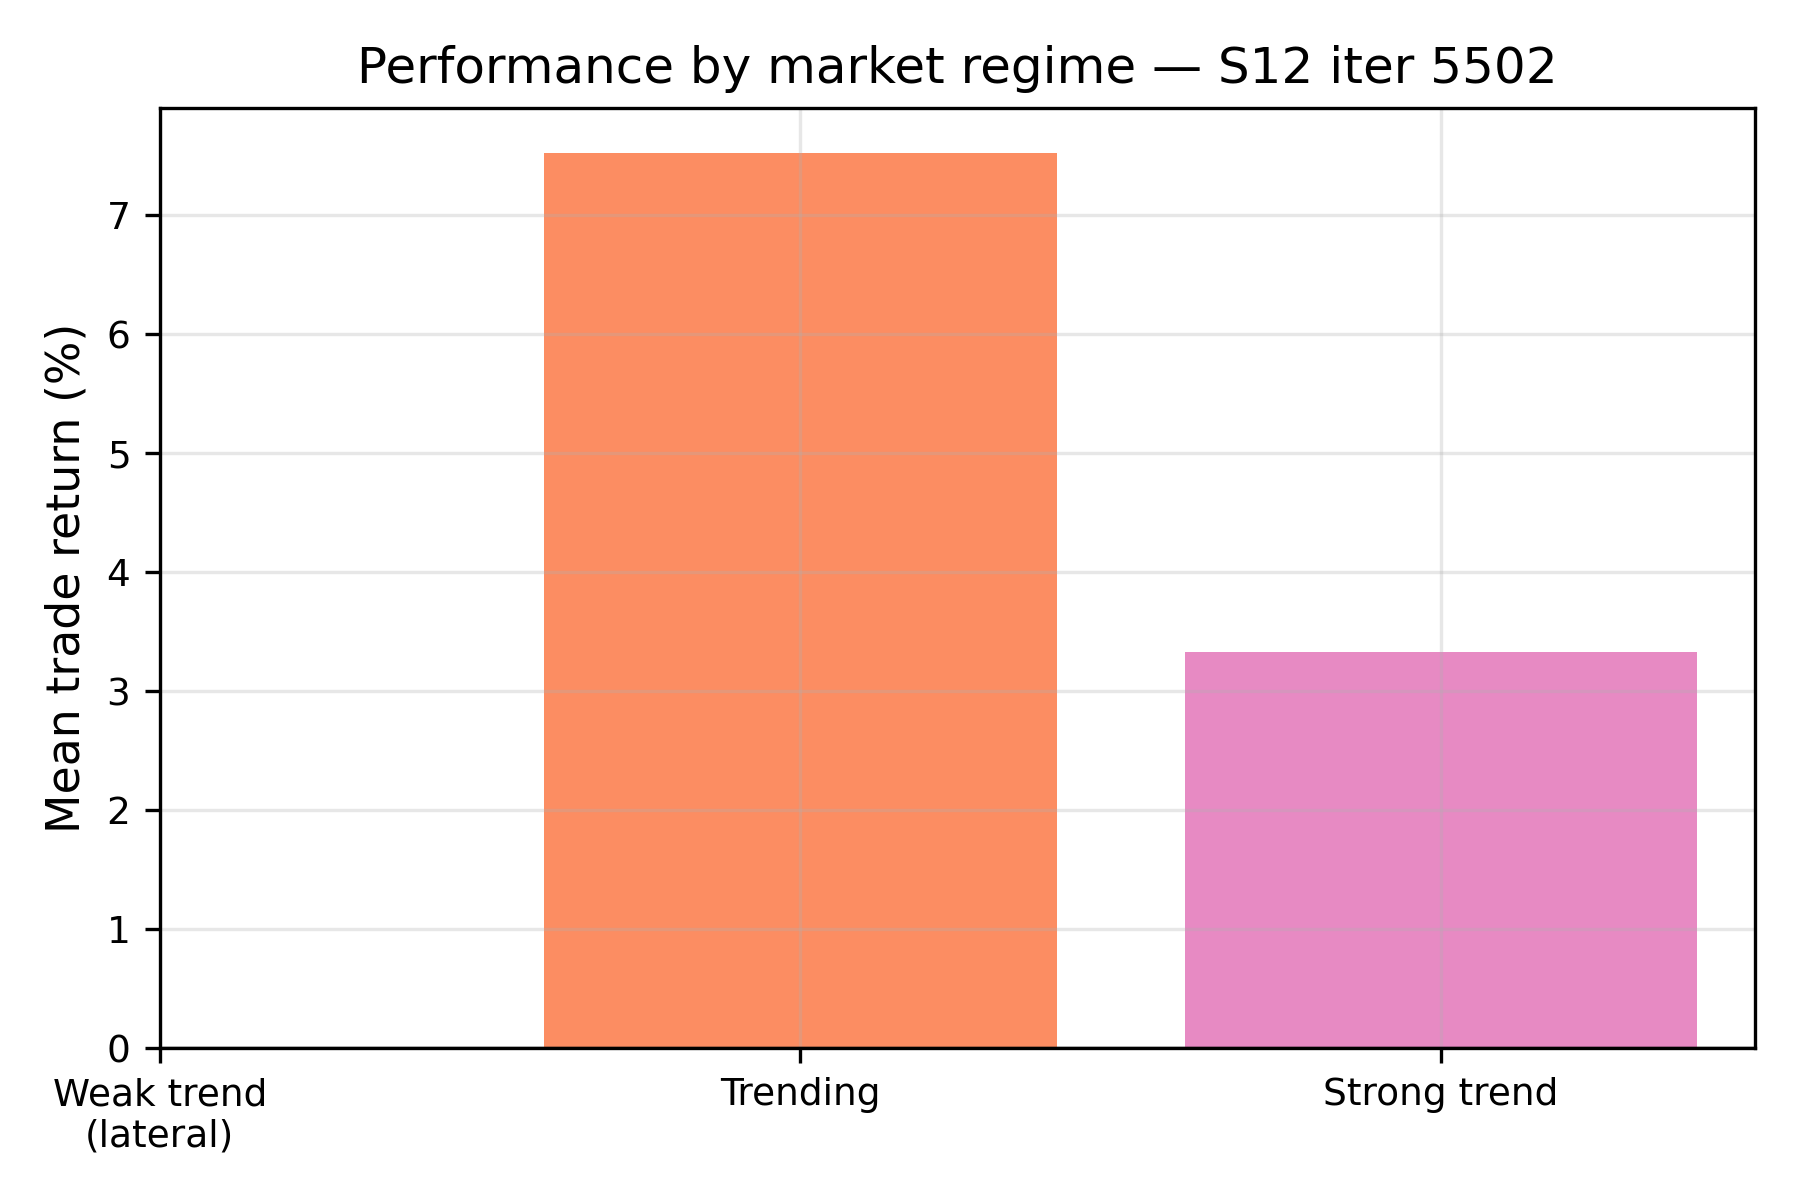
\includegraphics[width=0.85\textwidth]{figures/fig07_regime_analysis_s12_5502.png}
\caption{Performance by market regime --- S12 iter 5502.\label{fig7}}
\end{figure}

\textbf{Trade counts by ADX regime.} Table~\ref{tab:adx-regime-trades} reports the trade counts underlying the regime means.


\begin{longtable}[]{@{}
  >{\raggedright\arraybackslash}p{(\columnwidth - 14\tabcolsep) * \real{0.1000}}
  >{\raggedright\arraybackslash}p{(\columnwidth - 14\tabcolsep) * \real{0.1000}}
  >{\raggedleft\arraybackslash}p{(\columnwidth - 14\tabcolsep) * \real{0.1333}}
  >{\raggedleft\arraybackslash}p{(\columnwidth - 14\tabcolsep) * \real{0.1333}}
  >{\raggedleft\arraybackslash}p{(\columnwidth - 14\tabcolsep) * \real{0.1333}}
  >{\raggedleft\arraybackslash}p{(\columnwidth - 14\tabcolsep) * \real{0.1333}}
  >{\raggedleft\arraybackslash}p{(\columnwidth - 14\tabcolsep) * \real{0.1333}}
  >{\raggedleft\arraybackslash}p{(\columnwidth - 14\tabcolsep) * \real{0.1333}}@{}}
\caption{Trade counts by ADX regime}\label{tab:adx-regime-trades}\\
\toprule\noalign{}
\begin{minipage}[b]{\linewidth}\raggedright
ADX regime
\end{minipage} & \begin{minipage}[b]{\linewidth}\raggedright
Definition
\end{minipage} & \begin{minipage}[b]{\linewidth}\raggedleft
S11 iter 1077 trades
\end{minipage} & \begin{minipage}[b]{\linewidth}\raggedleft
S11 mean return (\%)
\end{minipage} & \begin{minipage}[b]{\linewidth}\raggedleft
S11 win rate (\%)
\end{minipage} & \begin{minipage}[b]{\linewidth}\raggedleft
S12 iter 5502 trades
\end{minipage} & \begin{minipage}[b]{\linewidth}\raggedleft
S12 mean return (\%)
\end{minipage} & \begin{minipage}[b]{\linewidth}\raggedleft
S12 win rate (\%)
\end{minipage} \\
\midrule\noalign{}
\endhead
\bottomrule\noalign{}
\endlastfoot
Weak trend & ADX \textless{} 20 & 0 & --- & --- & 0 & --- & --- \\
Trending & 20 $\leq$ ADX \textless{} 40 & 34 & 3.83 & 79.4 & 9 & 7.53 & 88.9 \\
Strong trend & ADX $\geq$ 40 & 16 & 3.18 & 75.0 & 126 & 3.33 & 69.8 \\
\end{longtable}

\emph{Note: S11 iter 1077 uses an ADX\_min filter of 22, so no trades occur in the weak-trend regime. S12 iter 5502 trades predominantly in strong-trend conditions, consistent with the ADX regime analysis in Figure 8.}

\subsection{Statistical rigor}\label{statistical-rigor}

All Sharpe ratios reported by the engine and in this section are computed from daily equity changes and annualized with $\sqrt{365}$, the standard convention for cryptocurrency markets. We compute this ratio in two ways. The \textbf{active-day Sharpe} uses only days with at least one closed position, discarding inactive days; it is the metric the backtest engine optimizes and is reported in Tables~\ref{tab:case-study-strategies} and~\ref{tab:s11-annual-performance} to match the engine output. The \textbf{calendar-time Sharpe} uses the full daily equity curve, including all zero-return inactive days; it is the more conservative headline metric because it reflects the experience of a continuously invested account. The calendar-time values are lower than the active-day values (see Table~\ref{tab:case-study-strategies}) and should be treated as the primary descriptive evidence for risk-adjusted performance.

Table~\ref{tab:bootstrap-dsr} reports active-day Sharpe ratios, bootstrap p-values, approximate Deflated Sharpe Ratios (DSR), and percentile bootstrap 95~\% confidence intervals for the three main case studies. Calendar-time Sharpe values are reported in Table~\ref{tab:case-study-strategies}. These statistics are intended as \textbf{descriptive diagnostics} of the strategies' holdout behavior, not as inferential guarantees or proof that the strategies will generalize. The bootstrap procedure tests the null hypothesis \(H_0: \mu \le 0\) against the one-sided alternative \(H_1: \mu > 0\), where \(\mu\) is the mean daily return on active trading days (days with at least one closed position). Both S11 models reject \(H_0\) at \(p < 0.0001\), and S12 rejects at \(p = 0.0012\). The approximate DSR values, which adjust for the raw number of trials in each season and for non-normality, remain positive: 11.78 for S11 iter 1077 and 3.24 for S12 iter 5502. These values should be interpreted as \textbf{optimistic upper bounds} because the DSR does not correct for the cross-season meta-search.

These statistics must be interpreted with their assumptions in mind. The bootstrap p-value relies on the sample of active trading days being representative of the strategy's future daily return distribution. This assumption is questionable for three reasons. First, the sample is conditional on days with at least one closed trade, so it omits inactive days and may overstate precision. Second, the number of active trading days is small (45--63), so the sampling distribution is noisy; the 95 \% bootstrap confidence intervals for the Sharpe ratio are wide (Table~\ref{tab:bootstrap-dsr}). Third, daily returns on active trading days are not independent: ACF(1) ranges from -0.24 to 0.18, and Jarque-Bera tests reject normality for the two S11 cases (p $\leq$ 0.0003). We therefore treat the p-values and DSR values as descriptive indicators rather than as exact frequentist probabilities or guarantees of future performance.

The approximate DSR is computed as follows. First, the variance of the Sharpe ratio under the null is adjusted for skewness and kurtosis following \citep{lo_2002}:

\[\widehat{\mathrm{Var}}(\mathrm{SR}) = \frac{1 - \hat{\gamma}_3 \cdot \mathrm{SR} + \frac{\hat{\gamma}_4 - 1}{4} \mathrm{SR}^2}{N - 1},\]

where \(\hat{\gamma}_3\) and \(\hat{\gamma}_4\) are the sample skewness and kurtosis and \(N\) is the number of active trading days with at least one closed position. The single-trial probability of observing a Sharpe at least as large as the reported value is \(p_1 = 1 - \Phi\big(\mathrm{SR} / \sqrt{\widehat{\mathrm{Var}}(\mathrm{SR})}\big)\), with \(\Phi\) the standard normal CDF. Under the simplifying assumption of \(K\) independent trials per season, the probability of observing at least one such Sharpe is \(p_K = 1 - (1 - p_1)^K\). The deflated Sharpe is then mapped back to the same probability level:

\[\mathrm{DSR} \approx \Phi^{-1}(1 - p_K) \cdot \sqrt{\widehat{\mathrm{Var}}(\mathrm{SR})}.\]

For S11 iter 1077, \(K = 3,797\) and \(N = 45\) active trading days; for S12 iter 5502, \(K = 9,957\) and \(N = 53\) active trading days. Because strategies share features and hyper-parameter ranges, the effective number of independent trials is smaller than the raw iteration count; therefore these DSR values should be interpreted as an upper bound on the correction rather than as exact Bailey--López de Prado probabilities. One difference is that Bailey and López de Prado \citep{bailey_2014} frame the Deflated Sharpe Ratio as the minimum significant Sharpe threshold that survives a multiple-testing correction, whereas the quantity reported here maps the Bonferroni-corrected p-value back onto the Sharpe scale for comparability with the raw Sharpe.

Finally, the single-season DSR and bootstrap p-values do not account for the outer meta-search across twelve seasons. Each season's gates and scoring weights were updated after observing prior holdout results, so the cross-season design itself consumes out-of-sample information. The reported DSR values are therefore optimistic bounds; a fully conservative accounting would require a protocol-level multiple-testing correction (e.g., \citep{romano_2005}) that is left for future work. We report the uncorrected diagnostics in Table~\ref{tab:bootstrap-dsr} with this caveat and do not use them to support claims of predictive skill.


\begin{longtable}[]{@{}
  >{\raggedright\arraybackslash}p{(\columnwidth - 18\tabcolsep) * \real{0.0769}}
  >{\raggedleft\arraybackslash}p{(\columnwidth - 18\tabcolsep) * \real{0.1026}}
  >{\raggedleft\arraybackslash}p{(\columnwidth - 18\tabcolsep) * \real{0.1026}}
  >{\raggedleft\arraybackslash}p{(\columnwidth - 18\tabcolsep) * \real{0.1026}}
  >{\raggedleft\arraybackslash}p{(\columnwidth - 18\tabcolsep) * \real{0.1026}}
  >{\raggedleft\arraybackslash}p{(\columnwidth - 18\tabcolsep) * \real{0.1026}}
  >{\raggedleft\arraybackslash}p{(\columnwidth - 18\tabcolsep) * \real{0.1026}}
  >{\raggedleft\arraybackslash}p{(\columnwidth - 18\tabcolsep) * \real{0.1026}}
  >{\raggedleft\arraybackslash}p{(\columnwidth - 18\tabcolsep) * \real{0.1026}}
  >{\raggedleft\arraybackslash}p{(\columnwidth - 18\tabcolsep) * \real{0.1026}}@{}}
\caption{Bootstrap p-values, approximate Deflated Sharpe Ratios, and 95~\% confidence intervals}\label{tab:bootstrap-dsr}\\
\toprule\noalign{}
\begin{minipage}[b]{\linewidth}\raggedright
Case
\end{minipage} & \begin{minipage}[b]{\linewidth}\raggedleft
Active-day Sharpe
\end{minipage} & \begin{minipage}[b]{\linewidth}\raggedleft
95 \% CI for Sharpe
\end{minipage} & \begin{minipage}[b]{\linewidth}\raggedleft
Bootstrap p-value (H$_0$: $\mu$ $\leq$ 0)
\end{minipage} & \begin{minipage}[b]{\linewidth}\raggedleft
95 \% CI for p-value
\end{minipage} & \begin{minipage}[b]{\linewidth}\raggedleft
Approx. DSR
\end{minipage} & \begin{minipage}[b]{\linewidth}\raggedleft
Active trading days
\end{minipage} & \begin{minipage}[b]{\linewidth}\raggedleft
Skewness
\end{minipage} & \begin{minipage}[b]{\linewidth}\raggedleft
Kurtosis
\end{minipage} & \begin{minipage}[b]{\linewidth}\raggedleft
ACF(1)
\end{minipage} \\
\midrule\noalign{}
\endhead
\bottomrule\noalign{}
\endlastfoot
S11 iter 1077 & 13.75 & {[}6.72, 25.83{]} & \textless{} 0.0001 & {[}0.0000, 0.0003{]} & 11.78 & 45 & -1.46 & 3.44 & -0.22 \\
S11 iter 1066 & 9.97 & {[}4.48, 17.25{]} & \textless{} 0.0001 & {[}0.0000, 0.0003{]} & 8.32 & 63 & -0.91 & 5.25 & -0.24 \\
S12 iter 5502 & 7.80 & {[}2.59, 13.65{]} & 0.0012 & {[}0.0005, 0.0019{]} & 3.24 & 53 & -0.20 & 1.97 & 0.18 \\
\end{longtable}

\emph{Note: The approximate DSR adjusts for the raw number of trials in the respective season (S11: 3,797; S12: 9,957) using the Bailey \& López de Prado (2014) formula. Because strategies share features and hyper-parameter ranges, the effective number of independent trials is smaller than the raw iteration count; the reported DSR values are therefore an optimistic upper bound on the correction. They also do not correct for the cross-season meta-search. Bootstrap uses 10,000 resamples with replacement of daily returns from active trading days with at least one closed position. The 95 \% confidence intervals for the Sharpe ratio are percentile bootstrap intervals; they are wide because the sample of active trading days is small. ACF(1) is the first-order autocorrelation of daily returns. Jarque-Bera tests reject normality for S11 iter 1077 (p = 0.0003) and S11 iter 1066 (p \textless{} 0.0001) but not for S12 iter 5502 (p = 0.26).}

\subsection{Temporal robustness and data-snooping considerations}\label{temporal-robustness-and-data-snooping-considerations}

The reported profitability in every calendar year (Tables~\ref{tab:s11-annual-performance} and~\ref{tab:s12-annual-performance}) is based on a small sample of annual blocks (five years per strategy) and a low number of trades per year (four to eighty-two), and should not be mistaken for independent out-of-sample evidence. The LLM's feature proposals and the season acceptance gates were both informed by earlier seasons, so the design itself consumes out-of-sample information through an outer meta-search loop. The single-season bootstrap p-values and DSR values in Table~\ref{tab:bootstrap-dsr} do not correct for this cross-season selection and are based on only 45--63 active trading days.

We therefore distinguish three levels of evidence, in decreasing order of strength:

\begin{enumerate}
\def\labelenumi{\arabic{enumi}.}
\item
  \textbf{Passive holdout:} the 2024--2025 years for S11 and S12 were never used by Optuna for parameter tuning. These are genuine holdout results within a season.
\item
  \textbf{Secondary selection holdout:} the January--March 2026 period for S11 was used to choose the production model from 30 re-evaluated candidates. It is therefore a post-selection observation, not an independent prospective test.
\item
  \textbf{Cross-season qualitative replication:} S12 (BTC/USDT) replicates the pipeline design after the lessons of S1--S11. This provides qualitative evidence of portability but is not a controlled ablation and does not rule out meta-overfitting.
\end{enumerate}

The evidence supports the narrower conclusion that the selected strategies are not trivial artifacts of in-sample curve fitting; it does not support unconditional claims about future performance.

Table~\ref{tab:temporal-robustness-windows} reports a temporal-robustness check on quarterly, semester, annual, and rolling 12-month windows. Annual windows are profitable for both strategies (Sharpe \textgreater{} 0 in 100 \% of windows), but shorter windows are noisier: only 59 \% and 60 \% of quarterly windows are positive for S11 and S12 respectively. This pattern is expected for a low-frequency strategy and cautions against over-interpreting any single short window.

\subsection{Temporal robustness across alternative window definitions}\label{table-10-temporal-robustness-across-alternative-window-definitions}

\begin{longtable}[]{@{}
  >{\raggedright\arraybackslash}p{(\columnwidth - 14\tabcolsep) * \real{0.1000}}
  >{\raggedright\arraybackslash}p{(\columnwidth - 14\tabcolsep) * \real{0.1000}}
  >{\raggedleft\arraybackslash}p{(\columnwidth - 14\tabcolsep) * \real{0.1333}}
  >{\raggedleft\arraybackslash}p{(\columnwidth - 14\tabcolsep) * \real{0.1333}}
  >{\raggedleft\arraybackslash}p{(\columnwidth - 14\tabcolsep) * \real{0.1333}}
  >{\raggedleft\arraybackslash}p{(\columnwidth - 14\tabcolsep) * \real{0.1333}}
  >{\raggedleft\arraybackslash}p{(\columnwidth - 14\tabcolsep) * \real{0.1333}}
  >{\raggedleft\arraybackslash}p{(\columnwidth - 14\tabcolsep) * \real{0.1333}}@{}}
\caption{Temporal robustness of Sharpe ratios across window definitions}\label{tab:temporal-robustness-windows}\\
\toprule\noalign{}
\begin{minipage}[b]{\linewidth}\raggedright
Window type
\end{minipage} & \begin{minipage}[b]{\linewidth}\raggedright
Case study
\end{minipage} & \begin{minipage}[b]{\linewidth}\raggedleft
N windows
\end{minipage} & \begin{minipage}[b]{\linewidth}\raggedleft
Mean Sharpe
\end{minipage} & \begin{minipage}[b]{\linewidth}\raggedleft
Std Sharpe
\end{minipage} & \begin{minipage}[b]{\linewidth}\raggedleft
Min Sharpe
\end{minipage} & \begin{minipage}[b]{\linewidth}\raggedleft
Max Sharpe
\end{minipage} & \begin{minipage}[b]{\linewidth}\raggedleft
Sharpe \textgreater{} 0 (\%)
\end{minipage} \\
\midrule\noalign{}
\endhead
\bottomrule\noalign{}
\endlastfoot
Quarterly & S11 BNB/USDT iter 1077 & 17 & 1.73 & 2.13 & --1.37 & 5.84 & 59 \\
Quarterly & S12 BTC/USDT iter 5502 & 20 & 0.83 & 2.08 & --2.54 & 3.40 & 60 \\
Semester & S11 BNB/USDT iter 1077 & 9 & 2.06 & 1.64 & --0.15 & ---$^a$ & 78 \\
Semester & S12 BTC/USDT iter 5502 & 10 & 1.39 & 1.21 & --0.61 & 2.83 & 80 \\
Annual & S11 BNB/USDT iter 1077 & 5 & 2.42 & 1.11 & 1.05 & ---$^a$ & 100 \\
Annual & S12 BTC/USDT iter 5502 & 5 & 1.39 & 0.56 & 0.70 & 2.22 & 100 \\
Rolling 12-month & S11 BNB/USDT iter 1077 & 5 & 2.42 & 1.11 & 1.05 & ---$^a$ & 100 \\
Rolling 12-month & S12 BTC/USDT iter 5502 & 5 & 1.39 & 0.56 & 0.70 & 2.22 & 100 \\
\end{longtable}

\emph{Note.} Quarterly and semester windows partition the available history; annual windows are calendar years; rolling 12-month windows start on 1 January of each available year. The number of windows differs because S11 spans 2022--2026 (with partial 2026 data) and S12 spans 2021--2025. Sharpe ratios are computed from daily equity changes annualized with \(\sqrt{365}\). $^a$~The Q1 2026 window for S11 is a post-selection observation used to choose the production model from 30 re-evaluated candidates (four trades) and is not an independent prospective test; its Sharpe is therefore omitted from the Max Sharpe summary.

\subsection{Ablation and baseline comparisons}\label{ablation-and-baseline-comparisons}

\subsubsection{Objective}

A natural question is whether the LLM proposal step adds value beyond a simpler random search over the same constrained space. We therefore compare the LLM-selected S12 BTC/USDT configuration (iter 5502) against two lightweight baselines that preserve the pipeline's validation, training, and backtesting infrastructure but remove the LLM from one dimension at a time.

\subsubsection{Design}

Table~\ref{tab:ablation-study} reports two baselines. The \emph{random SL/TP/threshold} baseline fixes the LLM-selected feature set and draws 200 \((\mathrm{SL}, \mathrm{TP}, \mathrm{threshold})\) triples at random from the same ranges used by Optuna. The \emph{random-feature} baseline fixes the final SL/TP/threshold values from the LLM configuration and draws eight random feature subsets from the catalog, training a fresh XGBoost classifier for each subset and then running a 30-trial random search over SL/TP/threshold. All backtests use \texttt{max\_pos\ =\ 5} and modeled costs of 0.20 \% fee plus 0.10 \% slippage; the 2024--2025 holdout window is never used for training or risk-parameter optimization.

\subsubsection{Results}

The random-parameter baseline has a mean holdout Sharpe of 0.90 across 200 draws, with 38 \% of draws exceeding a Sharpe of 1.0. The LLM-Optuna configuration lies at the 76th percentile of this distribution, so the risk-parameter optimization improves upon naive sampling but is not the dominant source of edge. The random-feature baseline is telling: its mean holdout Sharpe is 1.32 across eight random subsets, and the best random subset reaches 1.60, higher than the LLM-selected feature set's 1.15.

\subsubsection{Interpretation}

For this specific case study, the LLM did not identify a uniquely superior feature combination; many random combinations from the same leakage-free catalog perform comparably or better once the risk parameters are co-optimized. This does not mean the LLM is unnecessary---it generates the syntactically valid, catalog-compliant candidates that the validation layer then filters---but it does move the scientific contribution away from superhuman feature discovery and toward systematic validation and rejection of unsound candidates.

\subsubsection{Limitations}

Three caveats apply. First, the random-feature sample is small and the risk-parameter search for the random subsets used only 30 random trials, whereas the LLM configuration benefited from a full 120-trial Optuna study on the validation window. Second, the LLM's objective was the minimum validation Sharpe across sub-windows, not the mean holdout Sharpe reported here, so the comparison is not perfectly aligned. Third, an ablation that replaces the LLM with a completely random strategy generator---including random entry rules, model architectures, and risk parameters---would require a computational budget comparable to the full study and is left for future work. These results are therefore indicative rather than definitive.


\begin{longtable}[]{@{}
  >{\raggedright\arraybackslash}p{(\columnwidth - 12\tabcolsep) * \real{0.1200}}
  >{\raggedright\arraybackslash}p{(\columnwidth - 12\tabcolsep) * \real{0.1200}}
  >{\raggedright\arraybackslash}p{(\columnwidth - 12\tabcolsep) * \real{0.1200}}
  >{\raggedleft\arraybackslash}p{(\columnwidth - 12\tabcolsep) * \real{0.1600}}
  >{\raggedleft\arraybackslash}p{(\columnwidth - 12\tabcolsep) * \real{0.1600}}
  >{\raggedleft\arraybackslash}p{(\columnwidth - 12\tabcolsep) * \real{0.1600}}
  >{\raggedleft\arraybackslash}p{(\columnwidth - 12\tabcolsep) * \real{0.1600}}@{}}
\caption{Ablation study: random baselines versus LLM-selected configuration (S12 iter 5502)}\label{tab:ablation-study}\\
\toprule\noalign{}
\begin{minipage}[b]{\linewidth}\raggedright
Baseline
\end{minipage} & \begin{minipage}[b]{\linewidth}\raggedright
Fixed component
\end{minipage} & \begin{minipage}[b]{\linewidth}\raggedright
Varied component
\end{minipage} & \begin{minipage}[b]{\linewidth}\raggedleft
N configurations
\end{minipage} & \begin{minipage}[b]{\linewidth}\raggedleft
Mean holdout Sharpe (2024--2025)
\end{minipage} & \begin{minipage}[b]{\linewidth}\raggedleft
Best holdout Sharpe
\end{minipage} & \begin{minipage}[b]{\linewidth}\raggedleft
Sharpe \textgreater{} 1.0 (\%)
\end{minipage} \\
\midrule\noalign{}
\endhead
\bottomrule\noalign{}
\endlastfoot
LLM-selected & Features, SL, TP, threshold from S12 iter 5502 & --- & 1 & 1.15 & 1.15 & 100 \\
Random SL/TP/threshold & LLM-selected features & SL, TP, threshold uniform random & 200 & 0.90 $\pm$ 0.31 & 1.68 & 38 \\
Random features & SL=9.70, TP=9.12, Thr=0.890 & Feature subset uniform random & 8 & 1.32 $\pm$ 0.29 & 1.60 & 75 \\
\end{longtable}

\emph{Note: All backtests use \texttt{max\_pos\ =\ 5} and modeled costs of 0.20 \% fee + 0.10 \% slippage. The holdout window (2024--2025) was not used during training or Optuna optimization. Because the random-feature sample is small and the random search over risk parameters is coarser than the original Optuna study, these figures are indicative rather than definitive.}

\section{Discussion}\label{discussion}

\subsection{Interpretation of results}\label{interpretation-of-results}

The results show that a research system incorporating an LLM agent can generate directional candidates that survive strict validation when constrained by a leakage-free feature catalog and rigorous out-of-sample protocols. The marginal predictive power (AUC $\approx$ 0.53--0.57) is typical of short-term directional models in efficient markets; any economic value comes from combining weak signals with disciplined risk management and regime filtering, not from high-precision directional forecasts. Because the cross-season design updates objectives and gates after observing prior holdout results, the case studies should be read as \emph{evidence of the architecture's ability to screen out unsound candidates}, not as \emph{a forward-looking guarantee} of durable edge.

\textbf{Economic interpretation of the selected signals.} The S11 and S12 models rely on a small set of technical indicators. \emph{Stochastic RSI} and \emph{EMA differences} capture short- and medium-term momentum dynamics; in cryptocurrency markets, where retail flow and momentum strategies are common, these variables may proxy for lagged order-flow pressure \citep{sobreiro_2026}. \emph{ADX} measures trend strength and is used both as an entry filter and implicitly through the feature set, aligning the strategy with periods when directional persistence is more likely. \emph{Bollinger Band width} and \emph{ATR} quantify volatility compression and expansion; the volatility kill-switch prevents entries when realized volatility spikes, protecting the strategy from adverse gap risk. None of these signals is novel individually; the contribution is the automated, leakage-aware process that combines them and rejects configurations that fail out-of-sample gates.

\textbf{Value proposition relative to buy-and-hold.} Tables~\ref{tab:s11-benchmark} and~\ref{tab:s12-benchmark} show that the selected strategies underperform buy-and-hold in strong bull years. This is expected: the strategies are long-only, trade infrequently, and use stop-losses that cap upside during rapid rallies. The practical claim is therefore not total-return dominance, but drawdown control and positive returns in bear or sideways regimes. The S11 strategy's maximum drawdown of -6.74 \% versus -62.90 \% for buy-and-hold, and the S12 strategy's -8.0 \% versus -77.57 \%, show this risk-management profile. Whether this profile is attractive depends on the investor's marginal utility: a risk-averse holder seeking to limit downside may prefer the smoother equity curve, while an investor maximizing expected wealth would prefer the unlevered benchmark.

\textbf{The role of the LLM in light of the ablation is to generate, not to discover.} The ablation results in Section~\ref{ablation-and-baseline-comparisons} change how we interpret the LLM's role. Random feature subsets and random risk parameters can produce holdout performance comparable to, or even better than, the LLM-selected configuration in the S12 case study. This does not mean the LLM is unnecessary---it generates the syntactically valid, catalog-compliant candidates that the validation layer then filters---but it does mean that the scientific contribution is the validation and governance architecture, not a claim of superhuman feature discovery. The LLM functions here as a \textbf{high-volume proposal generator}; the pipeline converts a large volume of such proposals into a small set of testable strategies, and the statistical safeguards are what make that conversion credible. This finding is consistent with a recent post-mortem in the literature, where one highly automated, self-evolving trading system diverged sharply between validation and live performance \citep{chen_2025_redqueen}: the differentiator is not the strength of the proposal engine but the discipline with which its output is filtered.

\subsection{Limitations}\label{limitations}

The study has several limitations. First, the number of trades per strategy is low (tens to low-hundreds over several years), which increases sampling variance in daily return statistics; consequently, the bootstrap p-values in Table~\ref{tab:bootstrap-dsr}, though based on 10,000 resamples, should be interpreted with caution because they are computed from 45--63 non-i.i.d.~daily observations with wide confidence intervals. The reported Sharpe ratios are active-day ratios; calendar-time Sharpe, which includes all inactive days, is the more conservative headline metric and should be preferred for risk-adjusted comparisons.

Second, the January--March 2026 period for S11 is short (three months, four trades) and was used to select the production model from 30 re-evaluated candidates. It is therefore a secondary selection holdout rather than an independent prospective test, and its Sharpe should be treated as a noisy post-selection observation.

Third, the cross-season adaptive design consumes out-of-sample information. Because the human reviewer updated season objectives, acceptance gates, and scoring weights after observing prior holdout results, the sequence of seasons is best understood as a prolonged model-selection procedure rather than as a single pre-registered protocol tested once. The approximate DSR assumes independent trials and does not correct for this meta-search; because strategies also share features and hyper-parameter ranges, the effective number of independent trials is smaller than the raw iteration count and the reported deflated statistics are optimistic upper bounds.

Fourth, the set of reported results is subject to selection bias. Only candidates that passed the pipeline's gates are described in detail; many thousands of proposals were generated and rejected. The surviving strategies are therefore not a random sample of the search space, and their reported metrics overstate the expected performance of an arbitrary candidate drawn from the same generator.

Fifth, all results are simulated with modeled costs. Entry trades include 0.10 \% slippage, but stop-loss and take-profit exits are filled at the triggered level without additional slippage; live fills may therefore differ. Sixth, the multi-timeframe feature-merge module is imported at runtime from an external package (\texttt{features.technical}), although an internal copy is provided for audit and reproducibility. Seventh, the ablation study (Section~\ref{ablation-and-baseline-comparisons}) is limited to one accepted model and a modest number of random feature subsets; it supports the interpretation that validation is the dominant contribution, but it does not constitute a full factorial decomposition of every pipeline component. Eighth, the cryptocurrency market is highly non-stationary, and past performance may not generalize to future regimes.

Taken together, these limitations share a single root: the low trade count and the adaptive, cross-season search mean that our statistical diagnostics are interpreted as \emph{descriptive evidence that the pipeline rejects unsound candidates}, not as \emph{inferential guarantees} about the surviving ones. We therefore make no claim stronger than what a holdout-blind, leakage-controlled search can support. These results should be interpreted as evidence that the validation architecture can discipline candidate selection, not as proof of durable trading edge.

\subsection{Implications for practice}\label{implications-for-practice}

For quantitative researchers, the main implication is that LLMs can accelerate the strategy-proposal loop, but only if the surrounding infrastructure enforces temporal integrity and overfitting control. The LLM should not be trusted to avoid future leakage, to select hyper-parameters without validation, or to possess superior feature intuition; in our ablation, random feature subsets sometimes outperformed the LLM-selected configuration on the same holdout window. The value of the system lies in the validator-scorer-optimizer triad, not in the LLM alone.

For practitioners, the low-frequency nature of the accepted candidates, with win rates above 65\% on trades that clear the regime filter, is attractive because it minimizes transaction costs and operational risk. The regime filter, volatility kill-switch, and drawdown gates provide explicit risk controls within the research pipeline. However, the pipeline described here is an \textbf{offline research tool}; live deployment would require a separate online system with real-time data feeds, execution monitoring, position-sizing governance, and circuit breakers. We do not claim that the selected candidates are ready for live trading without that additional layer.

\subsection{Design principles}\label{design-principles}

Following the design-science paradigm in information-systems research \citep{hevner_2004}, the pipeline can be abstracted into three generalizable design principles that extend beyond the specific trading domain:

\begin{enumerate}
\def\labelenumi{\arabic{enumi}.}
\item
  \textbf{Season-structured autonomy with boundary human oversight.} The system delegates all routine experimentation to an autonomous agent within a season, while reserving high-level objective and gate updates for a human reviewer at season boundaries. This principle balances throughput with accountability and can be applied to any analytics workflow where the cost of human review per iteration is high but the cost of periodic strategic adjustment is low.
\item
  \textbf{Leakage-free feature constraints as a hard architectural invariant.} Temporal integrity is enforced by a restricted feature catalog, AST-based code validation, and explicit one-bar look-ahead lags for multi-timeframe merges. Treating leakage prevention as a non-negotiable design constraint, rather than as a post-hoc test, reduces the incidence of spurious strategies and lowers the multiple-testing burden.
\item
  \textbf{Multi-objective scoring that penalizes overfitting directly.} The composite score combines in-sample fit, holdout robustness, drawdown control, and validation-holdout decay. By optimizing a function that explicitly penalizes overfitting, the search is guided toward policies that generalize rather than toward policies that maximize backtest profit.
\end{enumerate}

These principles crystallize a position that recent work has begun to argue on independent grounds: that statistical rigor in AI-driven discovery is most effective when built into the structure of the search loop rather than applied as a downstream check \citep{benjamini_hochberg_1995}. The value of LLM-based proposal generation is therefore contingent on the surrounding analytical infrastructure---the LLM accelerates hypothesis generation, but the validation and scoring layers are what make the output credibly testable.

\subsection{Future work}\label{future-work}

Future directions include: (i) extending the system to portfolios of strategies and multiple assets; (ii) incorporating on-chain and sentiment features via a RAG layer; (iii) running a live paper-trading evaluation for at least 12 months; (iv) implementing the full Bailey-López de Prado DSR with cluster-based estimation of effective independent trials; and (v) exploring larger LLMs and code-specific models for strategy generation. A complementary direction is to evaluate the pipeline against the emerging verifiable, cost-aware benchmarks for quant-trading agents \citep{sun_2023_trademaster, sun_2023_prudex_compass}, which would allow the season-structured governance layer to be compared, under a common protocol, with alternative autonomous-agent designs.

\section{Conclusions}\label{conclusions}

We introduced a season-structured validation and governance architecture for autonomous prescriptive-algorithmic-trading pipelines. Within each season, a local LLM worked as a high-volume proposal generator; across season boundaries, a human reviewer updated objectives and gates, forming a mixed-initiative governance layer. A multi-layer validation system rejected unsound proposals before they reached the holdout. Evaluated across twelve experimental seasons and two cryptocurrencies, the pipeline produced 329 accepted strategies from 34,333 iterations and identified BNB/USDT and BTC/USDT candidates that remained profitable on holdout data when evaluated with conservative calendar-time Sharpe ratios. Because human-in-the-loop adjustments between seasons consume out-of-sample information, the reported case studies are descriptive evidence of the architecture's selective capacity, not independent prospective proof of future profitability. These outcomes depended on a restricted leakage-free feature catalog, a layered validation protocol, a holdout-blind optimization procedure, and explicit---but deliberately incomplete---statistical corrections for multiple testing.

The findings support a narrow claim: LLMs can accelerate prescriptive-analytics research only when embedded in a disciplined validation workflow. Because the ablation found no consistent statistical evidence that the LLM selects feature combinations better than random subsets from the same catalog, the contribution is the governance architecture itself---the systematic, leakage-aware rejection of candidates that would not survive out-of-sample scrutiny. The pipeline is a controlled experimental tool for hypothesis generation and systematic validation in data-rich domains, not a replacement for human judgment or a guarantee of future performance. Future work will focus on live paper-trading evaluation, protocol-level multiple-testing corrections, portfolio-level risk management, richer data modalities, and comparison against verifiable agent benchmarks.



\vspace{6pt}

% Declarations
\dataavailability{The code, experiment logs, and trained model artifacts supporting this study are openly available at Zenodo, DOI: 10.5281/zenodo.21160587 (\url{https://doi.org/10.5281/zenodo.21160587}), and at \url{https://github.com/pesobreiro/algo-autoresearch-paper}.

To reproduce the two case studies: (1) install the pinned Python environment listed in \texttt{requirements.txt}; (2) download 15-minute, 4-hour, and daily OHLCV bars for BNB/USDT and BTC/USDT from the Binance public API; (3) start the local Qwen2.5-7B-Instruct GGUF server via llama.cpp; (4) run \texttt{python main.py} for the desired season; (5) for the selected iterations, run \texttt{deployment/evaluate\_models.py} and \texttt{deployment/backtest\_deploy.py} using the saved model and parameters in \texttt{best\_models/season\_\{N\}/iter\_\{XXXX\}/}. A \texttt{download\_data.py} helper script that performs the exact Binance API calls used in this study is included in the repository. Byte-identical reproduction across operating systems is not guaranteed because of Numba JIT compilation and BLAS threading; the statistical conclusions, however, are robust to the residual non-determinism.}

\institutionalreview{This study uses publicly available historical market data and simulation-based backtesting. No human subjects, personally identifiable information, or animal data were involved. Ethical approval was therefore not required.}

\informedconsent{Not applicable. This research did not involve human subjects.}

\authorcontributions{Conceptualization, methodology, software, validation, formal analysis, investigation, data curation, writing --- original draft, writing --- review and editing, visualization, supervision: Pedro Sobreiro. Methodology, writing --- review and editing, supervision: Domingos Martinho. Methodology, writing --- review and editing: Pedro Ramos, Antonio Pratas. All authors have read and agreed to the published version of the manuscript.}

\conflictsofinterest{The authors declare no conflicts of interest. The research was conducted independently of any trading firm, exchange, or asset-management company.}

\funding{No external funding was received for this research.}

\acknowledgments{During the preparation of this manuscript, the authors used external AI-assisted tools for drafting, language polishing, and software-development support, and a locally deployed language model as part of the research methodology itself (see the Use of Artificial Intelligence Tools statement below for full details). All authors reviewed, tested, and edited every output and take full responsibility for the final manuscript, code, experimental design, statistical analysis, and scientific conclusions. No proprietary, personal, or non-public data were sent to external APIs.}

\useofartificialintelligence{During the preparation of this manuscript, large language model tools (Claude, Anthropic, San Francisco, CA, USA) were used to assist with text drafting, writing, and language polishing. Trinka (Crimson AI Pvt. Ltd., Mumbai, Maharashtra, India) was used for grammar and language correction. Large language model tools also assisted the authors during software development, including code drafting, debugging, and refactoring of the research pipeline (feature engineering, backtesting engine, and deployment scripts). Separately, and as a core component of the research methodology itself, a locally hosted large language model (Qwen2.5-7B-Instruct) was used as an autonomous strategy-proposal and code-generation agent within the season-structured research architecture described in Section 3; this use is not a development aid but the subject and method of the study, and it is fully described, validated, and audited as detailed in Sections 3.1, 3.4, and 3.6. In all cases, the authors reviewed, tested, and take full responsibility for the final code, experimental design, statistical analysis, and scientific conclusions reported in this paper.}


\begin{thebibliography}{999}
\bibitem{akiba_2019} Akiba, T., Sano, S., Yanase, T., Ohta, T., \& Koyama, M. (2019). Optuna: A next-generation hyperparameter optimization framework. \emph{Proceedings of the 25th ACM SIGKDD International Conference on Knowledge Discovery \& Data Mining, 2623--2631}. \url{https://doi.org/10.1145/3292500.3330701}.
\bibitem{allen_1999} Allen, F., \& Karjalainen, R. (1999). Using genetic algorithms to find technical trading rules. \emph{Journal of Financial Economics, 51(2), 245--271}. \url{https://doi.org/10.1016/S0304-405X(98)00052-X}.
\bibitem{almgren_2001} Almgren, R., \& Chriss, N. (2001). Optimal execution of portfolio transactions. \emph{Journal of Risk, 3(2), 5--39}. \url{https://doi.org/10.21314/JOR.2001.041}.
\bibitem{amershi_2019} Amershi, S., Weld, D., Vorvoreanu, M., Fourney, A., Nushi, B., Collisson, P., \ldots Horvitz, E. (2019). Guidelines for human-AI interaction. \emph{Proceedings of the 2019 CHI Conference on Human Factors in Computing Systems (CHI '19), Paper 3, 1--13}. \url{https://doi.org/10.1145/3290605.3300233}.
\bibitem{bailey_2014} Bailey, D. H., \& López de Prado, M. (2014). The Deflated Sharpe Ratio: Correcting for selection bias, backtest overfitting, and non-normality. \emph{Journal of Portfolio Management, 40(5), 94--107}. \url{https://doi.org/10.3905/jpm.2014.40.5.094}.
\bibitem{bailey_2017} Bailey, D. H., Borwein, J. M., López de Prado, M., \& Zhu, Q. J. (2017). The probability of backtest overfitting. \emph{Journal of Computational Finance, 20(4), 39--69}. \url{https://doi.org/10.21314/jcf.2016.322}.
\bibitem{bengio_2009} Bengio, Y., Louradour, J., Collobert, R., \& Weston, J. (2009). Curriculum learning. \emph{Proceedings of the 26th Annual International Conference on Machine Learning (ICML), 41--48}. \url{https://doi.org/10.1145/1553374.1553380}.
\bibitem{benjamini_hochberg_1995} Benjamini, Y., \& Hochberg, Y. (1995). Controlling the false discovery rate: a practical and powerful approach to multiple testing. \emph{Journal of the Royal Statistical Society, Series B, 57(1), 289--300}. \url{https://doi.org/10.1111/j.2517-6161.1995.tb02031.x}.
\bibitem{bertsimas_2020} Bertsimas, D., \& Kallus, N. (2020). From predictive to prescriptive analytics. \emph{Management Science, 66(3), 1025--1044}. \url{https://doi.org/10.1287/mnsc.2018.3253}.
\bibitem{brabazon_kampouridis_oneill_2020} Brabazon, A., Kampouridis, M., \& O'Neill, M. (2020). Applications of genetic programming to finance and economics: past, present, future. \emph{Genetic Programming and Evolvable Machines, 21(1), 33--53}. \url{https://doi.org/10.1007/s10710-019-09363-0}.
\bibitem{chen_2016} Chen, T., \& Guestrin, C. (2016). XGBoost: A scalable tree boosting system. \emph{Proceedings of the 22nd ACM SIGKDD International Conference on Knowledge Discovery and Data Mining, 785--794}. \url{https://doi.org/10.1145/2939672.2939785}.

\bibitem{chen_2021} Chen, M.; Tworek, J.; Jun, H.; Yuan, Q.; de Oliveira Pinto, H.P.; Kaplan, J.; Edwards, H.; Burda, Y.; Joseph, N.; Brockman, G.; Ray, A.; Puri, R.; Krueger, G.; Petrov, M.; Khlaaf, H.; Sastry, G.; Mishkin, P.; Chan, B.; Gray, S.; Ryder, N.; Pavlov, M.; Power, A.; Kaiser, L.; Bavarian, M.; Winter, C.; Tillet, P.; Such, F.P.; Cummings, D.; Plappert, M.; Chantzis, F.; Barnes, E.; Herbert-Voss, A.; Guss, W.H.; Nichol, A.; Paino, A.; Tezak, N.; Tang, J.; Babuschkin, I.; Balaji, S.; Jain, S.; Saunders, W.; Hesse, C.; Carr, A.N.; Leike, J.; Achiam, J.; Misra, V.; Morikawa, E.; Radford, A.; Knight, M.; Brundage, M.; Murati, M.; Mayer, K.; Welinder, P.; McGrew, B.; Amodei, D.; McCandlish, S.; Sutskever, I.; Zaremba, W. (2021). Evaluating large language models trained on code. \emph{arXiv preprint arXiv:2107.03374}. \url{https://doi.org/10.48550/arXiv.2107.03374}.
\bibitem{davenport_2007} Davenport, T. H., \& Harris, J. G. (2007). \emph{Competing on analytics: The new science of winning}. Harvard Business School Press.

\bibitem{detzel_novy_marx_velikov_2023} Detzel, A., Novy-Marx, R., \& Velikov, M. (2023). Model comparison with transaction costs. \emph{The Journal of Finance, 78(3), 1743--1775}. \url{https://doi.org/10.1111/jofi.13205}.
\bibitem{fang_2023_multi_agent} Fang, Y., Tang, Z., Ren, K., Liu, W., Zhao, L., Bian, J., Li, D., Zhang, W., Yu, Y., \& Liu, T.-Y. (2023). Learning Multi-Agent Intention-Aware Communication for Optimal Multi-Order Execution in Finance. In \emph{Proceedings of the 29th ACM SIGKDD Conference on Knowledge Discovery and Data Mining (KDD '23), 4003--4012}. \url{https://doi.org/10.1145/3580305.3599856}.

\bibitem{fu_2025} Fu, W. (2025). The New Quant: A Survey of Large Language Models in Financial Prediction and Trading. \emph{arXiv preprint arXiv:2510.05533}. \url{https://doi.org/10.48550/arXiv.2510.05533}.

\bibitem{gu_2020} Gu, S., Kelly, B., \& Xiu, D. (2020). Empirical asset pricing via machine learning. \emph{The Review of Financial Studies, 33(5), 2223--2273}. \url{https://doi.org/10.1093/rfs/hhaa009}.
\bibitem{hamilton_1989} Hamilton, J. D. (1989). A new approach to the economic analysis of nonstationary time series and the business cycle. \emph{Econometrica, 57(2), 357--384}. \url{https://doi.org/10.2307/1912559}.
\bibitem{harvey_2015} Harvey, C. R., \& Liu, Y. (2015). Backtesting. \emph{Journal of Portfolio Management, 42(1), 13--28}. \url{https://doi.org/10.3905/jpm.2015.42.1.013}.
\bibitem{harvey_2016} Harvey, C. R., Liu, Y., \& Zhu, H. (2016). \ldots and the cross-section of expected returns. \emph{The Review of Financial Studies, 29(1), 5--68}. \url{https://doi.org/10.1093/rfs/hhv059}.
\bibitem{hevner_2004} Hevner, A. R., March, S. T., Park, J., \& Ram, S. (2004). Design science in information systems research. \emph{MIS Quarterly, 28(1), 75--105}. \url{https://doi.org/10.2307/25148625}.
\bibitem{horvitz_1999} Horvitz, E. (1999). Principles of mixed-initiative user interfaces. \emph{Proceedings of the SIGCHI Conference on Human Factors in Computing Systems (CHI '99), 159--166}. \url{https://doi.org/10.1145/302979.303030}.
\bibitem{hutter_2019} Hutter, F., Kotthoff, L., \& Vanschoren, J. (Eds.). (2019). \emph{Automated Machine Learning: Methods, Systems, Challenges. Springer}. \url{https://doi.org/10.1007/978-3-030-05318-5}.
\bibitem{jadhav_mirza_2025} Jadhav, A., \& Mirza, V. (2025). Large Language Models in equity markets: applications, techniques, and insights. \emph{Frontiers in Artificial Intelligence, 8, 1608365}. \url{https://doi.org/10.3389/frai.2025.1608365}.
\bibitem{jobson_1981} Jobson, J. D., \& Korkie, B. M. (1981). Performance hypothesis testing with the Sharpe and Treynor measures. \emph{The Journal of Finance, 36(4), 889--908}. \url{https://doi.org/10.1111/j.1540-6261.1981.tb04891.x}.
\bibitem{kaufman_2012} Kaufman, S., Rosset, S., Perlich, C., \& Stitelman, O. (2012). Leakage in data mining: Formulation, detection, and avoidance. \emph{ACM Transactions on Knowledge Discovery from Data, 6(4), 1--21}. \url{https://doi.org/10.1145/2382577.2382579}.
\bibitem{kou_2024} Kou, Z., Yu, H., Luo, J., Peng, J., Li, X., Liu, C., Dai, J., Chen, L., Han, S., \& Guo, Y. (2025). Automate Strategy Finding with LLM in Quant Investment. In \emph{Findings of the Association for Computational Linguistics: EMNLP 2025, 18517--18533}. \url{https://doi.org/10.18653/v1/2025.findings-emnlp.1005}.
\bibitem{ledoit_2008} Ledoit, O., \& Wolf, M. (2008). Robust performance hypothesis testing with the Sharpe ratio. \emph{Journal of Empirical Finance, 15(5), 850--859}. \url{https://doi.org/10.1016/j.jempfin.2008.03.002}.
\bibitem{liu_2021} Liu, X.-Y., Yang, H., Gao, J., \& Wang, C. D. (2021). FinRL: Deep reinforcement learning framework to automate trading in quantitative finance. \emph{Proceedings of the Second ACM International Conference on AI in Finance, Article 1}. \url{https://doi.org/10.1145/3490354.3494366}.
\bibitem{lo_2002} Lo, A. W. (2002). The statistics of Sharpe ratios. \emph{Financial Analysts Journal, 58(4), 36--52}. \url{https://doi.org/10.2469/faj.v58.n4.2453}.
\bibitem{prado_2018} L\u00f3pez de Prado, M. (2018). \emph{Advances in financial machine learning}. Wiley.

\bibitem{romano_2005} Romano, J. P., \& Wolf, M. (2005). Stepwise multiple testing as formalized data snooping. \emph{Econometrica, 73(4), 1237--1282}. \url{https://doi.org/10.1111/j.1468-0262.2005.00615.x}.
\bibitem{sullivan_1999} Sullivan, R., Timmermann, A., \& White, H. (1999). Data-snooping, technical trading rule performance, and the bootstrap. \emph{The Journal of Finance, 54(5), 1647--1691}. \url{https://doi.org/10.1111/0022-1082.00166}.
\bibitem{sullivan_2001} Sullivan, R., Timmermann, A., \& White, H. (2001). Dangers of data mining: The case of calendar effects in stock returns. \emph{Journal of Econometrics, 105(1), 249--286}. \url{https://doi.org/10.1016/S0304-4076(01)00077-X}.
\bibitem{white_2000} White, H. (2000). A reality check for data snooping. \emph{Econometrica, 68(5), 1097--1126}. \url{https://doi.org/10.1111/1468-0262.00152}.
\bibitem{hansen_2005} Hansen, P. R. (2005). A test for superior predictive ability. \emph{Journal of Business \& Economic Statistics, 23(4), 365--380}. \url{https://doi.org/10.1198/073500105000000063}.
\bibitem{shmueli_2011} Shmueli, G., \& Koppius, O. R. (2011). Predictive analytics in information systems research. \emph{MIS Quarterly, 35(3), 553--572}. \url{https://doi.org/10.2307/23042796}.
\bibitem{sobreiro_2026} Sobreiro, P., Martinho, D., Martins, R., \& Vardasca, R. (2026). Multi-timeframe feature engineering for Bitcoin market prediction: A price-level-agnostic machine learning approach. \emph{Forecasting, 8(3), 40}. \url{https://doi.org/10.3390/forecast8030040}.
\bibitem{sun_2023_rl_survey} Sun, S., Wang, R., \& An, B. (2023). Reinforcement learning for quantitative trading. \emph{ACM Transactions on Intelligent Systems and Technology, 14(3), 44:1--44:29}. \url{https://doi.org/10.1145/3582560}.
\bibitem{sun_2023_trademaster} Sun, S., Qin, M., Zhang, W., Xia, H., Zong, C., Ying, J., Xie, Y., Zhao, L., Wang, X., \& An, B. (2023). TradeMaster: A Holistic Quantitative Trading Platform Empowered by Reinforcement Learning. In \emph{Advances in Neural Information Processing Systems (NeurIPS 2023), Datasets and Benchmarks Track}.
\bibitem{sun_2023_prudex_compass} Sun, S., Qin, M., Wang, X., \& An, B. (2023). PRUDEX-Compass: Towards Systematic Evaluation of Reinforcement Learning in Financial Markets. \emph{Transactions on Machine Learning Research}.
\bibitem{sutton_2018} Sutton, R. S., \& Barto, A. G. (2018). \emph{Reinforcement learning: An introduction (2nd ed.)}. MIT Press.

\bibitem{wang_2023} Wang, S., Yuan, H., Zhou, L., Ni, L. M., Shum, H. Y., \& Guo, J. (2025). Alpha-GPT: Human-AI Interactive Alpha Mining for Quantitative Investment. In \emph{Proceedings of the 2025 Conference on Empirical Methods in Natural Language Processing: System Demonstrations, 196--206}. \url{https://doi.org/10.18653/v1/2025.emnlp-demos.14}.
\bibitem{wei_2022} Wei, J., Wang, X., Schuurmans, D., Bosma, M., Ichter, B., Xia, F., Chi, E., Le, Q. V., \& Zhou, D. (2022). Chain-of-thought prompting elicits reasoning in large language models. \emph{Advances in Neural Information Processing Systems, 35, 24824--24837}. \url{https://doi.org/10.48550/arXiv.2201.11903}.
\bibitem{wilder_1978} Wilder, J. W. (1978). \emph{New Concepts in Technical Trading Systems}. Trend Research.

\bibitem{yao_2023} Yao, S., Zhao, J., Yu, D., Du, N., Shafran, I., Narasimhan, K., \& Cao, Y. (2023). ReAct: Synergizing reasoning and acting in language models. \emph{Proceedings of the 11th International Conference on Learning Representations (ICLR 2023)}. \url{https://openreview.net/forum?id=WE_vluYUL-X}.
\bibitem{yu_2023_synergistic_alpha} Yu, S., Xue, H., Ao, X., Pan, F., He, J., Tu, D., \& He, Q. (2023). Generating Synergistic Formulaic Alpha Collections via Reinforcement Learning. In \emph{Proceedings of the 29th ACM SIGKDD Conference on Knowledge Discovery and Data Mining (KDD '23), 5476--5486}. \url{https://doi.org/10.1145/3580305.3599831}.
\bibitem{yuan_2024} Yuan, H., Wang, S., \& Guo, J. (2024). Alpha-GPT 2.0: Human-in-the-loop AI for quantitative investment. \emph{arXiv preprint arXiv:2402.09746}. \url{https://doi.org/10.48550/arXiv.2402.09746}.
\bibitem{zhang_2024} Zhang, C.; Liu, X.; Zhang, Z.; Jin, M.; Li, L.; Wang, Z.; Hua, W.; Shu, D.; Zhu, S.; Jin, X.; Li, S.; Du, M.; Zhang, Y. (2024). When AI meets finance (StockAgent): Large language model-based stock trading in simulated real-world environments. \emph{arXiv preprint arXiv:2407.18957}. \url{https://doi.org/10.48550/arXiv.2407.18957}.
\bibitem{zhang_2024_finagent} Zhang, W., Zhao, L., Xia, H., Sun, S., Sun, J., Qin, M., Li, X., Zhao, Y., Zhao, Y., Cai, X., et al. (2024). A Multimodal Foundation Agent for Financial Trading: Tool-Augmented, Diversified, and Generalist. In \emph{Proceedings of the 30th ACM SIGKDD Conference on Knowledge Discovery and Data Mining (KDD '24), 4314--4325}. \url{https://doi.org/10.1145/3637528.3671801}.
\bibitem{zhang_2025} Zhang, D., Jiang, Z., Ji, Q., Liu, H., Wang, T., \& Stefanidis, A. (2025). LLM-guided evolutionary strategy generation for quantitative trading. \emph{2025 IEEE International Conference on Systems, Man, and Cybernetics (SMC), 3665--3670}. \url{https://doi.org/10.1109/SMC58881.2025.11343400}.
\bibitem{chen_2025_redqueen} Chen, Y. (2025). The Red Queen's Trap: Limits of Deep Evolution in High-Frequency Trading. \emph{arXiv preprint arXiv:2512.15732}. \url{https://doi.org/10.48550/arXiv.2512.15732}.
\bibitem{deeparies_2025} Kim, J., Yi, H., Gim, M., Choi, D., \& Kang, J. (2025). DeepAries: Adaptive Rebalancing Interval Selection for Enhanced Portfolio Selection. In \emph{Proceedings of the 34th ACM International Conference on Information and Knowledge Management (CIKM '25), 8 pages}. \url{https://doi.org/10.1145/3746252.3761572}.
\bibitem{yao_zheng_2026} Yao, J., \& Zheng, Z. (2026). Beyond Agent Architecture: Execution Assumptions and Reproducibility in LLM-Based Trading Systems. \emph{arXiv preprint arXiv:2606.08285}. \url{https://doi.org/10.48550/arXiv.2606.08285}.
\bibitem{zhang_maringer_2016} Zhang, J., \& Maringer, D. (2016). Using a genetic algorithm to improve recurrent reinforcement learning for equity trading. \emph{Computational Economics, 47(4), 551--567}. \url{https://doi.org/10.1007/s10614-015-9491-z}.
\end{thebibliography}

\end{document}
